
\chapter{Neural Networks}\label{chapter:neural_nets}
%\textit{Draft chapter from Torralba, Isola, Freeman}

\section{Introduction}
Neural networks are functions loosely modeled on the brain. In the brain, we have billions of neurons that connect to one another. Each neuron can be thought of as a node in a graph, and the edges are the connections from one neuron to the next (\fig{\ref{fig:neural_nets:fig1_net}}). The edges are directed; electrical signals propagate in just one direction along the wires in the brain.

\begin{figure}[h]
\centerline{
\begin{tikzpicture}%[>=spaced latex]
\draw [thick] (0,0) circle [radius=0.2];
\draw [thick] [nn_edge] (0.2,0) -- (0.8,-0.4);
\draw [thick] [nn_edge] (0.2,0) -- (0.8,0.4);
\draw [thick] (1,-0.4) circle [radius=0.2];
\draw [thick] (1,0.4) circle [radius=0.2];
\draw [thick] [nn_edge] (1.2,-0.4) -- (1.8,-0.4);
\draw [thick] [nn_edge] (1.2,0.4) -- (1.8,0.4);
\draw [thick] [nn_edge] (1.2,-0.4) -- (1.8,0.4);
\draw [thick] [nn_edge] (1.2,0.4) -- (1.8,-0.4);
\draw [thick] (2,-0.4) circle [radius=0.2];
\draw [thick] (2,0.4) circle [radius=0.2];
\draw [thick] [nn_edge] (2.2,-0.4) -- (2.8,0);
\draw [thick] [nn_edge] (2.2,0.4) -- (2.8,0);
\draw [thick] (3.0,0) circle [radius=0.2];
\end{tikzpicture}
}
\caption{A neural network can be drawn as a directed graph.}
\label{fig:neural_nets:fig1_net}
\end{figure}


Outgoing edges are called axons and incoming edges are called dendrites. A neuron fires, sending a pulse down its axon, when the incoming pulses, from the dendrites, exceed a threshold. 

\section{The Perceptron: A Simple Model of a Single Neuron}
Let's consider a neuron, shaded in gray, that has four inputs and one output (\fig{\ref{fig:neural_nets:perceptron_fig2}}).
\begin{figure}[h]
\centerline{
\begin{tikzpicture}[>=spaced latex]
\draw [thick] (0,-0.75) circle [radius=0.2];
\draw [thick] (0,-0.25) circle [radius=0.2];
\draw [thick] (0,0.25) circle [radius=0.2];
\draw [thick] (0,0.75) circle [radius=0.2];
\draw [thick] [nn_edge] (0.2,-0.75) -- (0.8,-0.1);
\draw [thick] [nn_edge] (0.2,-0.25) -- (0.8,-0.05);
\draw [thick] [nn_edge] (0.2,0.25) -- (0.8,0.05);
\draw [thick] [nn_edge] (0.2,0.75) -- (0.8,0.1);
\draw [thick, fill=gray_neuron] (1,0) circle [radius=0.2];
\draw [thick] [nn_edge] (1.2,0) -- (1.8,0);
\draw [thick] (2.0,0) circle [radius=0.2];
\end{tikzpicture}
}
\caption{Perceptron.}
\label{fig:neural_nets:perceptron_fig2}
\end{figure}

A simple model for this neuron is the \index{Perceptron}{\bf perceptron}. A perceptron is a neuron with $n$ inputs $\{x_i\}_{i=1}^n$ and one output $y$, that maps inputs to outputs according to the following equations:
\begin{align}
    z = f(\mathbf{x}) &= \sum_{i=1}^n w_i x_i + b = \mathbf{w}^\transpose\mathbf{x} + b &\triangleleft \quad \text{linear layer}\\
    g(z) &= \begin{cases}
    1, &\text{if} \quad z > 0\\
    0,              & \text{otherwise}
\end{cases} &\triangleleft \quad \text{activation function}\label{eqn:neural_nets:perceptron_activation}\\
    y &= g(f(\mathbf{x})) &\triangleleft \quad \text{perceptron}
\end{align}

In words, we take a weighted sum of the inputs and, if that sum exceeds a threshold (here 0), the neuron fires (outputs a 1). The function $f$ is called a \index{Linear layer}{\bf linear layer} because it computes a linear function of the inputs, $\mathbf{w}^\transpose\mathbf{x}$, plus a \index{Bias}\textbf{bias}, b. The function $g$ is called the \index{Activation function}{\bf activation function} because it decides whether the neuron activates (fires).\marginnote{Mathematically, $f$ is an affine function, but by convention we call it a ``linear layer.'' One way to think of it is $f$ is a linear function of $\begin{bmatrix}\mathbf{x}\\ 1\end{bmatrix}$.}[-0.8cm]

\subsection{The Perceptron as a Classifier}
People got excited about perceptrons in the late 1950s because it was shown that they can learn to classify data~\cite{rosenblatt1958perceptron}. Let's see how that works. We will consider a perceptron with two inputs, $x_1$ and $x_2$, and one output, $y$. Let the incoming connection weights be $w_1 = 2$, $w_2 = 1$, and $b=0$. The values of $z$ and $y$, as a function of $x_1$ and $x_2$, are shown in \fig{\ref{fig:neural_nets:perceptron_as_classifier}}.

\begin{figure}[h]
\centerline{

\noindent\hspace{0.05\linewidth}
\begin{minipage}{.25\linewidth}

\begin{tikzpicture}[>=spaced latex]
\draw [thick] (0,-0.4) circle [radius=0.3] node {$x_2$};
\draw [thick] (0,0.4) circle [radius=0.3] node {$x_1$};
\draw [thick] [nn_edge] (0.3,-0.4) -- (1.0,-0.05) node[midway,below] {$w_2$};
\draw [thick] [nn_edge] (0.3,0.4) -- (1.0,0.05) node[midway,above] {$w_1$};
\draw [thick, fill=gray_neuron] (1.3,0) circle [radius=0.3] node {$z$};
\draw [thick] [nn_edge] (1.6,0) -- (2.3,0);
\draw [thick] (2.6,0) circle [radius=0.3] node {$y$};
\end{tikzpicture}

\end{minipage}
\begin{minipage}{.68\linewidth}

\begin{tikzpicture}
\begin{axis}[name=plot1, view={0}{90}, xmin=-1, xmax=1, ymin=-1, ymax=1, 
width=0.5\linewidth, xlabel=$x_1$, ylabel=$x_2$, 
title=$z$,
axis equal image,
x label style={at={(axis description cs:0.5,-0.17)}},
y label style={at={(axis description cs:-0.17,0.5)}},
]
	\addplot3[surf, shader=interp, domain=-1:1] {2*x+y};
	\end{axis}
%\end{tikzpicture}
%\end{minipage}
%\begin{minipage}{.30\linewidth}
%\begin{tikzpicture}
\begin{axis}[name=plot2, at=(plot1.right of south east), xshift=30, view={0}{90}, xmin=-1, xmax=1, ymin=-1, ymax=1, 
width=0.5\linewidth, xlabel=$x_1$, ylabel=$x_2$,
title=$y$,
colorbar,
colorbar style={
        ytick={-3.0,-2.0,-1.0,0,1.0,2.0,3.0},
        yticklabel style={
            align=right
        },
        width=5.0
    },
axis equal image,
x label style={at={(axis description cs:0.5,-0.17)}},
y label style={at={(axis description cs:-0.17,0.5)}},
%ymajorticks=false
]
    \addplot3[surf, shader=interp, domain=-1:1] {2*x+y};
	%\addplot[fill] {-2*x} -- cycle;
	\addplot[fill, index of colormap={5 of viridis}, color=.] coordinates 
		{(-1,-1) (0.5,-1) (-0.5,1) (-1,1)} --cycle;
	\addplot[fill, index of colormap={10 of viridis}, color=.] coordinates 
		{(0.5,-1) (1,-1) (1,1) (-0.5,1)} --cycle;
	\end{axis}
\end{tikzpicture}

\end{minipage}
}
\caption{Value of hidden unit ($z$) and output unit ($y$) in a perceptron, as a function of the input data.}
\label{fig:neural_nets:perceptron_as_classifier}
\end{figure}

Notice that $y$ takes on values 0 or 1, so you can think of this as a classifier that assigns a class label of 1 to the upper-right half of the plotted region.

\subsection{Learning with a Perceptron}
So a perceptron acts like a classifier, but how can we use it to learn? The idea is that given data, $\{\mathbf{x}^{(i)}, y^{(i)}\}_{i=1}^N$, we will adjust the weights $\mathbf{w}$ and the bias $b$, in order to minimize a classification loss, $\mathcal{L}$, that scores number of misclassifications:
\begin{align}
    \mathbf{w}^*, b^* = \argmin_{\mathbf{w}, b} \frac{1}{N}\sum_{i=1}^N \mathcal{L}(\mathbf{w}^\transpose\mathbf{x}^{(i)} + b, y^{(i)})\label{eqn:neural_nets:perceptron_learning_problem}
\end{align}
In \fig{\ref{fig:neural_nets:fitting_a_perceptron}}, this optimization process corresponds to shifting and rotating the \textbf{decision boundary}, until you find a line that separates data labeled as $y = 0$ from data labeled as $y = 1$.
\begin{figure}[h]
%\centerline{
%\noindent\hspace{0.05\linewidth}
\begin{minipage}{0.32\linewidth}
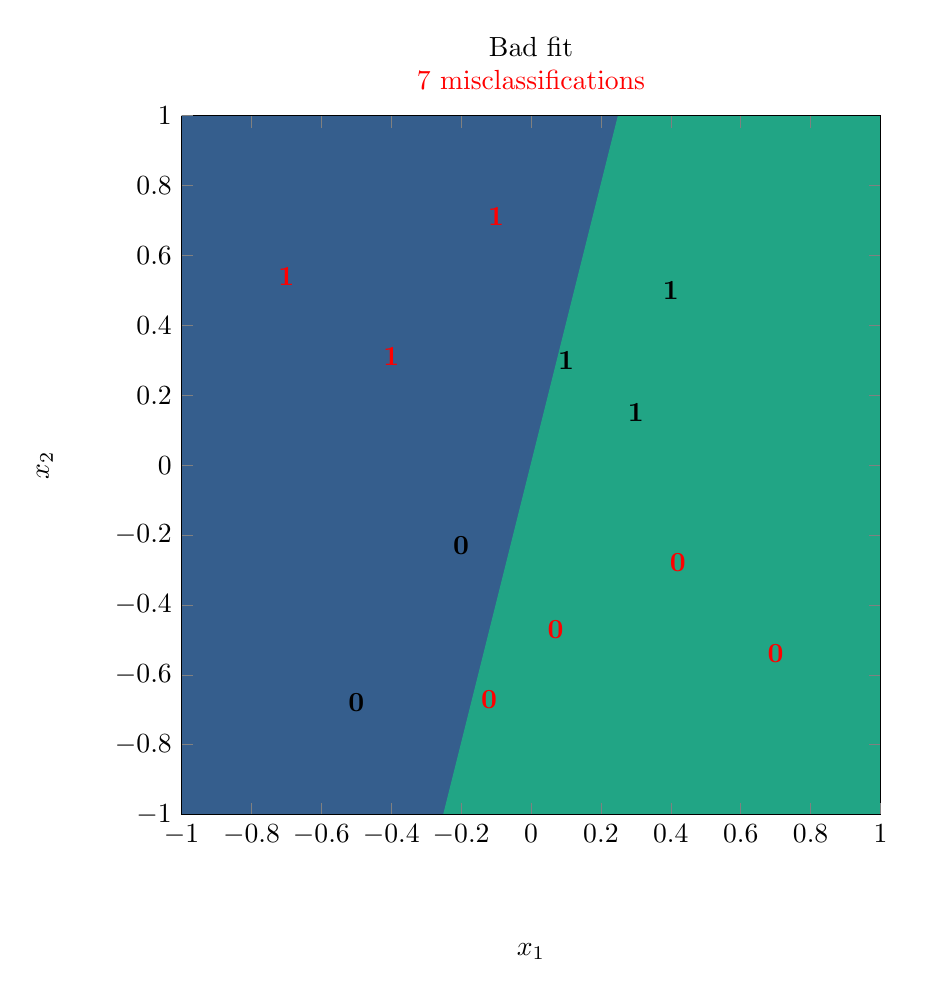
\begin{tikzpicture}
\begin{axis}[view={0}{90}, xmin=-1, xmax=1, ymin=-1, ymax=1, 
width=1.0\linewidth, xlabel=$x_1$, ylabel=$x_2$,
align=center,
title={Bad fit\\\color{red} 7 misclassifications},
axis equal image,
x label style={at={(axis description cs:0.5,-0.17)}},
y label style={at={(axis description cs:-0.17,0.5)}},
scatter/classes={%
    pos_correct={mark=text, text mark={\bf 1}},%
    pos_incorrect={mark=text, text mark={\bf \color{red} 1}},%
    neg_correct={mark=text, text mark={\bf 0}},%
    neg_incorrect={mark=text, text mark={\bf \color{red} 0}}}]
%
\addplot3[surf, shader=interp, domain=-1:1] {2*x+y};
	%\addplot[fill] {-2*x} -- cycle;
	\addplot[fill, index of colormap={5 of viridis}, color=.] coordinates 
		{(-1,-1) (-1,1) (0.25,1) (-0.25,-1)} --cycle;
	\addplot[fill, index of colormap={10 of viridis}, color=.] coordinates 
		{(0.25,1) (1,1) (1,-1) (-0.25,-1)} --cycle;

\addplot[scatter,only marks,%
    scatter src=explicit symbolic]%
table[meta=label] {
x y label
0.1 0.3 pos_correct
0.3 0.15 pos_correct
0.4 0.5 pos_correct
-0.1 0.71 pos_incorrect
-0.4 0.31 pos_incorrect
-0.7 0.54 pos_incorrect
%
-0.5 -0.68 neg_correct
-0.2 -0.23 neg_correct
-0.12 -0.67 neg_incorrect
0.07 -0.47 neg_incorrect
0.42 -0.28 neg_incorrect
0.7 -0.54 neg_incorrect
    };
\end{axis}
\end{tikzpicture}
\end{minipage}
%
%
\begin{minipage}{0.32\linewidth}
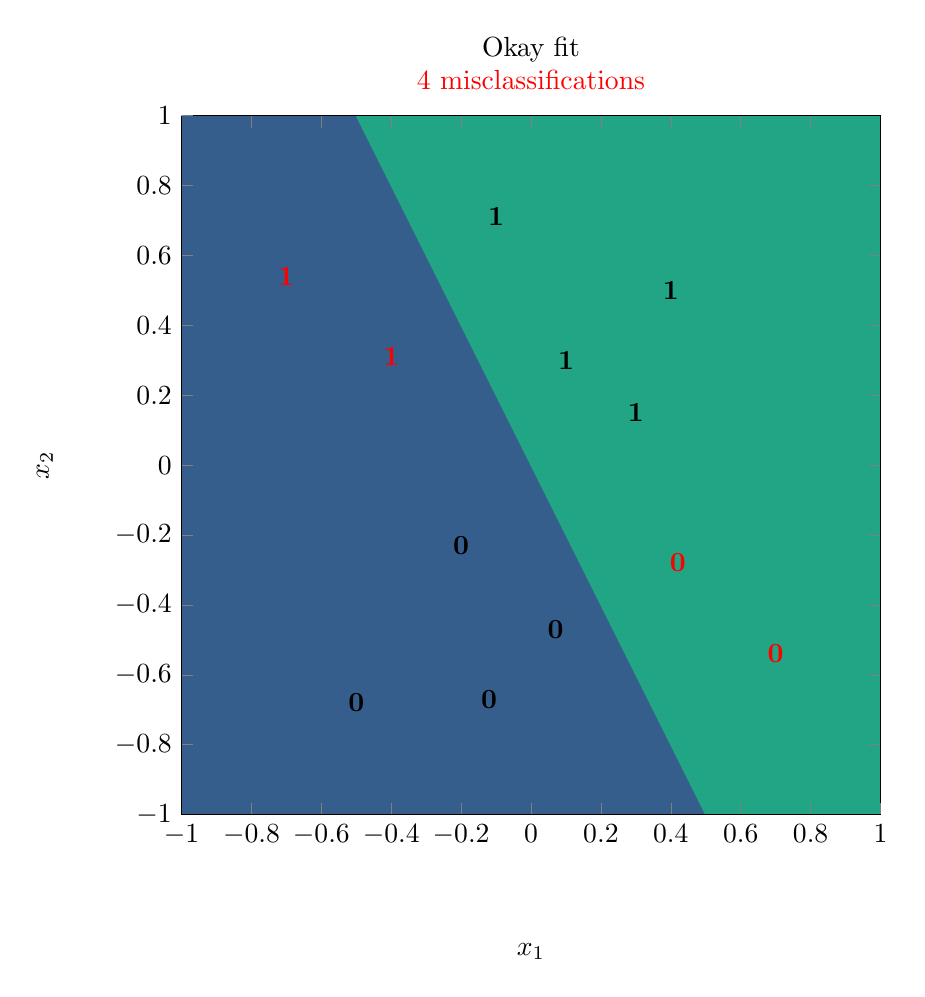
\begin{tikzpicture}
\begin{axis}[view={0}{90}, xmin=-1, xmax=1, ymin=-1, ymax=1, 
width=1.0\linewidth, xlabel=$x_1$, ylabel=$x_2$,
align=center,
title={Okay fit\\\color{red} 4 misclassifications},
axis equal image,
x label style={at={(axis description cs:0.5,-0.17)}},
y label style={at={(axis description cs:-0.17,0.5)}},
scatter/classes={%
    pos_correct={mark=text, text mark={\bf 1}},%
    pos_incorrect={mark=text, text mark={\bf \color{red} 1}},%
    neg_correct={mark=text, text mark={\bf 0}},%
    neg_incorrect={mark=text, text mark={\bf \color{red} 0}}}]
%
\addplot3[surf, shader=interp, domain=-1:1] {2*x+y};
	%\addplot[fill] {-2*x} -- cycle;
	\addplot[fill, index of colormap={5 of viridis}, color=.] coordinates 
		{(-1,-1) (0.5,-1) (-0.5,1) (-1,1)} --cycle;
	\addplot[fill, index of colormap={10 of viridis}, color=.] coordinates 
		{(0.5,-1) (1,-1) (1,1) (-0.5,1)} --cycle;
%
\addplot[scatter,only marks,%
    scatter src=explicit symbolic]%
table[meta=label] {
x y label
0.1 0.3 pos_correct
0.3 0.15 pos_correct
0.4 0.5 pos_correct
-0.1 0.71 pos_correct
-0.4 0.31 pos_incorrect
-0.7 0.54 pos_incorrect
%
-0.12 -0.67 neg_correct
-0.2 -0.23 neg_correct
-0.5 -0.68 neg_correct
0.07 -0.47 neg_correct
0.42 -0.28 neg_incorrect
0.7 -0.54 neg_incorrect
    };
\end{axis}
\end{tikzpicture}
\end{minipage}
%
%
\begin{minipage}{0.32\linewidth}
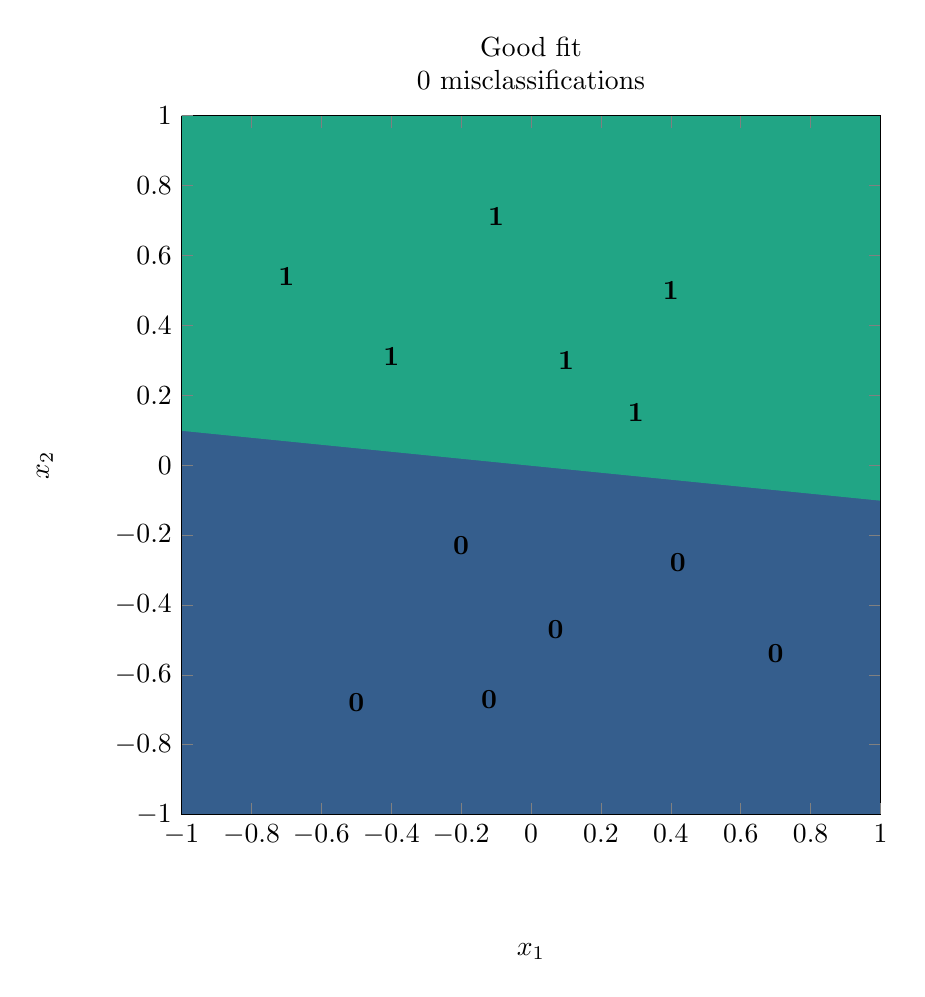
\begin{tikzpicture}
\begin{axis}[view={0}{90}, xmin=-1, xmax=1, ymin=-1, ymax=1, 
width=1.0\linewidth, xlabel=$x_1$, ylabel=$x_2$,
align=center,
title={Good fit\\0 misclassifications},
axis equal image,
x label style={at={(axis description cs:0.5,-0.17)}},
y label style={at={(axis description cs:-0.17,0.5)}},
scatter/classes={%
    pos_correct={mark=text, text mark={\bf 1}},%
    pos_incorrect={mark=text, text mark={\bf \color{red} 1}},%
    neg_correct={mark=text, text mark={\bf 0}},%
    neg_incorrect={mark=text, text mark={\bf \color{red} 0}}}]
%
\addplot3[surf, shader=interp, domain=-1:1] {2*x+y};
	%\addplot[fill] {-2*x} -- cycle;
	\addplot[fill, index of colormap={5 of viridis}, color=.] coordinates 
		{(-1,-1) (1,-1) (1,-0.1) (-1,0.1)} --cycle;
	\addplot[fill, index of colormap={10 of viridis}, color=.] coordinates 
		{(-1,0.1) (-1,1) (1,1) (1,-0.1)} --cycle;
%
\addplot[scatter,only marks,%
    scatter src=explicit symbolic]%
table[meta=label] {
x y label
0.1 0.3 pos_correct
0.3 0.15 pos_correct
0.4 0.5 pos_correct
-0.1 0.71 pos_correct
-0.4 0.31 pos_correct
-0.7 0.54 pos_correct
%
-0.12 -0.67 neg_correct
-0.2 -0.23 neg_correct
-0.5 -0.68 neg_correct
0.07 -0.47 neg_correct
0.42 -0.28 neg_correct
0.7 -0.54 neg_correct
    };
\end{axis}
\end{tikzpicture}
\end{minipage}
\caption{Different possible decision surfaces of a perceptron.}
\label{fig:neural_nets:fitting_a_perceptron}
\end{figure}

You might be wondering, what's the exact optimization algorithm that will find the best line that separates the classes? The original perceptron paper proposed one particular algorithm, the ``perceptron learning algorithm.'' This was an optimizer tailored to the specific structure of the perceptron. Older papers on neural nets are full of specific learning rules for specific architectures: the delta rule, the Rescorla-Wagner model, and so forth~\cite{rescorla1972theory}. Nowadays we rarely use these special-purpose algorithms. Instead, we use \textit{general-purpose} optimizers like gradient descent (for differentiable objectives) or zeroth-order methods (for nondifferentiable objectives). The next chapter will cover the backpropagation algorithm, which is a general-purpose gradient-based optimizer that applies to essentially all neural networks we will see in this book (but, note that for the perceptron objective, because it has a nondifferentiable threshold function, we would instead opt for a zeroth order optimizer).

\section{Multilayer Perceptrons}
Perceptrons can solve linearly separable binary classification problems, but they are otherwise rather limited. For one, they only produce a single output. What if we want multiple outputs? We can achieve this by adding edges that fan out after the perceptron (\fig{\ref{fig:neural_nets:fan_out}}).
%What if we want to output probabilities for $k$ different classes?
%What if we want to output continuous values rather than just zeros and ones? This brings us to the general purpose neuron that is the building block of almost all modern neural nets:
\begin{figure}[h]
\centerline{
\begin{tikzpicture}[>=spaced latex]
\draw [thick] (0,-0.75) circle [radius=0.2] node[label={$\mathbf{x}$}] at (0,0.85) {};
\draw [thick] (0,0.1) node {$\vdots$};
\draw [thick] (0,0.75) circle [radius=0.2];
\draw [thick] [nn_edge] (0.2,-0.75) -- (0.8,-0.1);
\draw [thick] [nn_edge] (0.2,0.0) -- (0.8,0.0);
\draw [thick] [nn_edge] (0.2,0.75) -- (0.8,0.1);
\draw [thick, fill=gray_neuron] (1,0) circle [radius=0.2]  node[label={$z$}] at (1.0,0.2) {};
\draw [thick] [nn_edge] (1.2,0.0) -- (1.8,0.0);
\draw [thick, fill=gray_neuron] (2.0,0) circle [radius=0.2]  node[label={$h$}] at (2.0,0.2) {};
\draw [thick] [nn_edge] (2.2,-0.1) -- (2.8,-0.75);
\draw [thick] [nn_edge] (2.2,0.0) -- (2.8,0.0);
\draw [thick] [nn_edge] (2.2,0.1) -- (2.8,0.75);
\draw [thick] (3.0,-0.75) circle [radius=0.2] node[label={$\mathbf{y}$}] at (3.0,0.8) {};
\draw [thick] (3.0,0.1)  node {$\vdots$};
\draw [thick] (3.0,0.75) circle [radius=0.2];
\end{tikzpicture}
}
\caption{Multiple outputs fan out from a neuron.}
\label{fig:neural_nets:fan_out}
\end{figure}

This network maps an input {\bf layer} of data $\mathbf{x}$ to a layer of outputs {\bf y}. The neurons in between inputs and outputs are called {\bf hidden units}, shaded in gray. Here, $z$ is a \index{Preactivaton unit}{\bf preactivation} hidden unit and $h$ is a \index{Postactivation unit}{\bf postactivation} hidden unit, that is, $h = g(z)$ where $g(\cdot)$ is an activation function like in \eqn{\ref{eqn:neural_nets:perceptron_activation}}.

More commonly we might have many hidden units in stack, which we call a \index{Hidden layer}{\bf hidden layer} (\fig{\ref{fig:neural_nets:MLP1}}).
%The diagram above has one hidden layer, with a single neuron $h$, called a {\bf hidden unit}
\begin{figure}[h]
\centerline{
\begin{tikzpicture}[>=spaced latex]
\draw [thick] (0,-0.75) circle [radius=0.2] node[label={$\mathbf{x}$}] at (0,0.85) {};
\draw [thick] (0,0.1) node {$\vdots$};
\draw [thick] (0,0.75) circle [radius=0.2];

\draw [thick,dotted] (0.33,-1.2)  .. controls (0.43,-1.05) .. (0.43,-0.9);
\draw (0.4,-1.45) node {$\mathbf{W}_1$};

\draw [thick] [nn_edge] (0.2,-0.75) -- (0.8,-0.1);
\draw [thick] [nn_edge] (0.2,-0.75) -- (0.8,-0.75);
\draw [thick] [nn_edge] (0.2,-0.75) -- (0.8,0.75);
\draw [thick] [nn_edge] (0.2,-0.1) -- (0.8,-0.75);
\draw [thick] [nn_edge] (0.2,0.0) -- (0.8,0.0);
\draw [thick] [nn_edge] (0.2,0.1) -- (0.8,0.75);
\draw [thick] [nn_edge] (0.2,0.75) -- (0.8,0.75);
\draw [thick] [nn_edge] (0.2,0.75) -- (0.8,-0.75);
\draw [thick] [nn_edge] (0.2,0.75) -- (0.8,0.1);
\draw [thick, fill=gray_neuron] (1,0.75) circle [radius=0.2]  node[label={$\mathbf{z}$}] at (1.0,0.85) {};
\draw [thick] (1,0.1) node {$\vdots$};
\draw [thick, fill=gray_neuron] (1,-0.75) circle [radius=0.2];
\draw [thick] [nn_edge] (1.2,0.75) -- (1.8,0.75);
\draw [thick] [nn_edge] (1.2,0.0) -- (1.8,0.0);
\draw [thick] [nn_edge] (1.2,-0.75) -- (1.8,-0.75);
\draw [thick, fill=gray_neuron] (1,0.75) circle [radius=0.2]  node[label={$\mathbf{h}$}] at (2.0,0.85) {};
\draw [thick, fill=gray_neuron] (2.0,0.75) circle [radius=0.2];
\draw [thick] (2.0,0.1) node {$\vdots$};
\draw [thick, fill=gray_neuron] (2.0,-0.75) circle [radius=0.2];

\draw [thick,dotted] (2.33,-1.2)  .. controls (2.43,-1.05) .. (2.43,-0.9);
\draw (2.4,-1.45) node {$\mathbf{W}_2$};

\draw [thick] [nn_edge] (2.2,-0.75) -- (2.8,-0.75);
\draw [thick] [nn_edge] (2.2,-0.75) -- (2.8,0.75);
\draw [thick] [nn_edge] (2.2,-0.75) -- (2.8,0.0);
\draw [thick] [nn_edge] (2.2,-0.1) -- (2.8,-0.75);
\draw [thick] [nn_edge] (2.2,0.0) -- (2.8,0.0);
\draw [thick] [nn_edge] (2.2,0.1) -- (2.8,0.75);
\draw [thick] [nn_edge] (2.2,0.75) -- (2.8,0.75);
\draw [thick] [nn_edge] (2.2,0.75) -- (2.8,-0.75);
\draw [thick] [nn_edge] (2.2,0.75) -- (2.8,0.0);
\draw [thick] (3.0,-0.75) circle [radius=0.2] node[label={$\mathbf{y}$}] at (3.0,0.8) {};
\draw [thick] (3.0,0.1)  node {$\vdots$};
\draw [thick] (3.0,0.75) circle [radius=0.2];
\end{tikzpicture}
}
\caption{Mutilayer perceptron.}
\label{fig:neural_nets:MLP1}
\end{figure}
\marginnote{How many layers does this net have? Some texts will say two [$\mathbf{W}_1$, $\mathbf{W}_2$], others three [$\mathbf{x}$, $\{\mathbf{z}, \mathbf{h}\}$, $\mathbf{y}$], others four [$\mathbf{x}$, $\mathbf{z}$, $\mathbf{h}$, $\mathbf{y}$]. We must get comfortable with the ambiguity.}[2cm]
% In biology, $h_i$ and $y_i$ are two parts of a single neuron, but often in artificial neural nets we call each node in these diagrams a ``neuron".

Because this network has multiple layers of neurons, and because each neuron in this net acts as a perceptron, we call it a \index{Multilayer perceptron}\textbf{multilayer perceptron} (\textbf{MLP}). The equation for this MLP is:
\begin{align}
    \mathbf{z} &= \mathbf{W}_1\mathbf{x} + \mathbf{b}_1 &\triangleleft \quad \text{linear layer}\\
    \mathbf{h} &= g(\mathbf{z}) &\triangleleft \quad \text{activation function}\\
    \mathbf{y} &= \mathbf{W}_2\mathbf{h} + \mathbf{b}_2 &\triangleleft \quad \text{linear layer}
\end{align}
In general, MLPs can be constructed with any number of layers following this pattern: linear layer, activation function, linear layer, activation function, and so on.

The activation function $g$ could be the threshold function like in \eqn{\ref{eqn:neural_nets:perceptron_activation}}, but more generally it can be any pointwise nonlinearity, that is, $g(\mathbf{h}) = [\tilde{g}(h_1), \ldots, \tilde{g}(h_N)]$ and $\tilde{g}$ is any nonlinear function that maps $\mathbb{R} \rightarrow \mathbb{R}$.

Beyond MLPs, this kind of sequence (linear layer, pointwise nonlinearity, linear layer, pointwise nonlinearity, and so on) is the prototpyical motif in almost all neural networks, including most we will see later in this book.

\section{Activations Versus Parameters}

When working with deep nets it's useful to distinguish \emph{activations} and \emph{parameters}. The activations are the values that the neurons take on, $[\mathbf{x}, \mathbf{z}_1, \mathbf{h}_1, \ldots, \mathbf{z}_{L-1}, \mathbf{h}_{L-1}, \mathbf{y}]$; slightly abusing notation, we use this term for both preactivation function neurons and postactivation function neurons. The activations are the neural representations of the data being processed. Often, we will not worry about distinguishing between inputs, hidden units, and outputs to the net, and simply refer to all data and neural activations in a network, layer by layer, as a sequence $[\mathbf{x}_0, \ldots, \mathbf{x}_L]$, in which case $\mathbf{x}_0$ is the raw input data.

\marginnote{
A multilayer network is a sequence of transformations $f_1, \ldots, f_L$ that produce a series of activations $\mathbf{x}_1, \ldots, \mathbf{x}_L$: 
\\[6pt]
\begin{center}
\begin{tikzpicture}
    \def\layerheight{0.8}
    \def\layerwidth{1.3}
    \def\blockheight{1.8}
    \def\blockwidth{1.3}
    % draw f's
    \foreach \x in {0,1,2,3} {
        \pgfmathsetmacro{\index}{int(\x+1)}
        \draw [fill=white] (2*\layerwidth*\x,-0.5*\blockheight) rectangle ++(\blockwidth,\blockheight) node[midway] {$f_{\index}(\mathbf{x}_{\x}, \theta_{\index})$};
    }
    % draw x's
    \foreach \x in {0,1,2,3} {
        \pgfmathsetmacro{\index}{int(\x+1)}
        \draw (2*\layerwidth*\x+0.5*\blockwidth-\layerwidth,0) node {$\mathbf{x}_\x$}; 
    }
    % draw arrows
    %\foreach \x in {0,1,2,3,4,5,6} {
    \foreach \x in {0,2,4,6} {
        %\draw [thick] [nn_edge] (0,\layerheight*\x+\blockheight) -- (0,\layerheight*\x+\layerheight);
        \draw [thick] [nn_edge] (\layerwidth*\x+\blockwidth,0) -- (\layerwidth*\x+\blockwidth+0.4*\layerwidth,0);
        \draw [thick] [nn_edge] (\layerwidth*\x+\blockwidth+0.65*\layerwidth-2*\layerwidth,0) -- (\layerwidth*\x+\blockwidth+\layerwidth-2*\layerwidth,0);
    }
    %\draw [thick] [nn_edge] (0,\layerheight*-1+\blockheight) -- (0,\layerheight*-1+\layerheight);
    \draw (7*\layerwidth+0.5*\blockwidth,0) node {$\mathbf{y}$}; 
\end{tikzpicture}
\end{center}
}[-2.2cm]

Conversely, parameters are the weights and biases of the network. These are the variables being learned. Both activations and parameters are tensors of variables.

Often we think of a layer as a function $\mathbf{x}_{l+1} = f_{l+1}(\mathbf{x}_l)$, but we can also make the parameters explicit and think of each layer as a function:
\begin{align}
    \mathbf{x}_{l+1} = f_{l+1}(\mathbf{x}_{l}, \theta_{l+1})
\end{align}
That is, each layer takes the activations from the previous layer, as well as parameters of the current layer as input, and produces activations of the next layer. Varying either the input activations or the input parameters will affect the output of the layer. From this perspective, anything we can do with parameters, we can do with activations instead, and vice versa, and that is the basis for a lot of applications and tricks. For example, while normally we learn the values of the parameters, we could instead hold the parameters fixed and learn the values of the activations that achieve some objective. In fact, this is what is done in many methods such as network prompting, adversarial attacks, and network visualization, which we will see in more detail in later chapters.
% \subsection{Data vs parameters}

% When working with deep nets it's useful to distinguish \emph{data} and \emph{parameters}. The ``data" are the values that the nodes take on, $[\mathbf{x}, \mathbf{z}_1, \mathbf{h}_1, \ldots, \mathbf{z}_{L-1}, \mathbf{h}_{L-1}, \mathbf{y}]$. It may seem strange at first to call all these variables data, but the idea is that all these values are \textit{representations} of the signal being processed. The inputs $\mathbf{x}$ are a ``raw" representation of the signal whereas later layers of neurons are transformed representations. Often, we will not worry about distinguishing between inputs, hidden units, and outputs, and simply refer to the data in a network, layer by layer, as a sequence $[\mathbf{x}_1, \ldots, \mathbf{x}_L]$.

% Parameters are the weights and biases mentioned above. These are the variables being learned. Both data and parameters are tensors of variables.

% Often we think of a layer as a function $\mathbf{x}_{l+1} = f_{l+1}(\mathbf{x}_l)$, but we can also make the parameters explicit and think of each layer as a function:
% \begin{align}
%     \mathbf{x}_{l+1} = f_{l+1}(\mathbf{x}_{l}, \theta_{l+1})
% \end{align}
% That is, each layer takes the data from the previous layer, as well as parameters of the current layer as input, and produces data of the next layer. Varying either the input data or the input parameters will affect the output of the layer. From this perspective, anything we can do with parameters, we can do with data instead, and vice versa, and that is the basis for a lot of applications and tricks. For example, while normally we learn the values of the parameters, we could instead hold the parameters fixed and learn the values of the data that achieve some objective. In fact this is what is done in applications such as style transfer, adversarial attacks, and network visualization, which we will see in more detail in later chapters.


\subsection{Fast Activations and Slow Parameters}%{\small [Advanced topic]}}
So what's different about activations versus parameters? One way to think about it is that activations are \textit{fast} functions of a data\textit{point}: they are the result of a few layers of processing this datapoint. Parameters are \textit{also} functions of the data (they are learned from data) but they are \textit{slow} functions of data\textit{sets}: the parameters are arrived at via an optimization procedure over a whole dataset. So, both activations and parameters are statistics of the data, that is, information extracted about about the data that organizes or summarizes it. The parameters are a kind of metasummary since they specify a functional transformation that produces activations from data, and activations themselves are a summary of the data. \Fig{\ref{fig:neural_nets:params_vs_activations}} shows how this looks.
\begin{figure}[h]
\centerline{
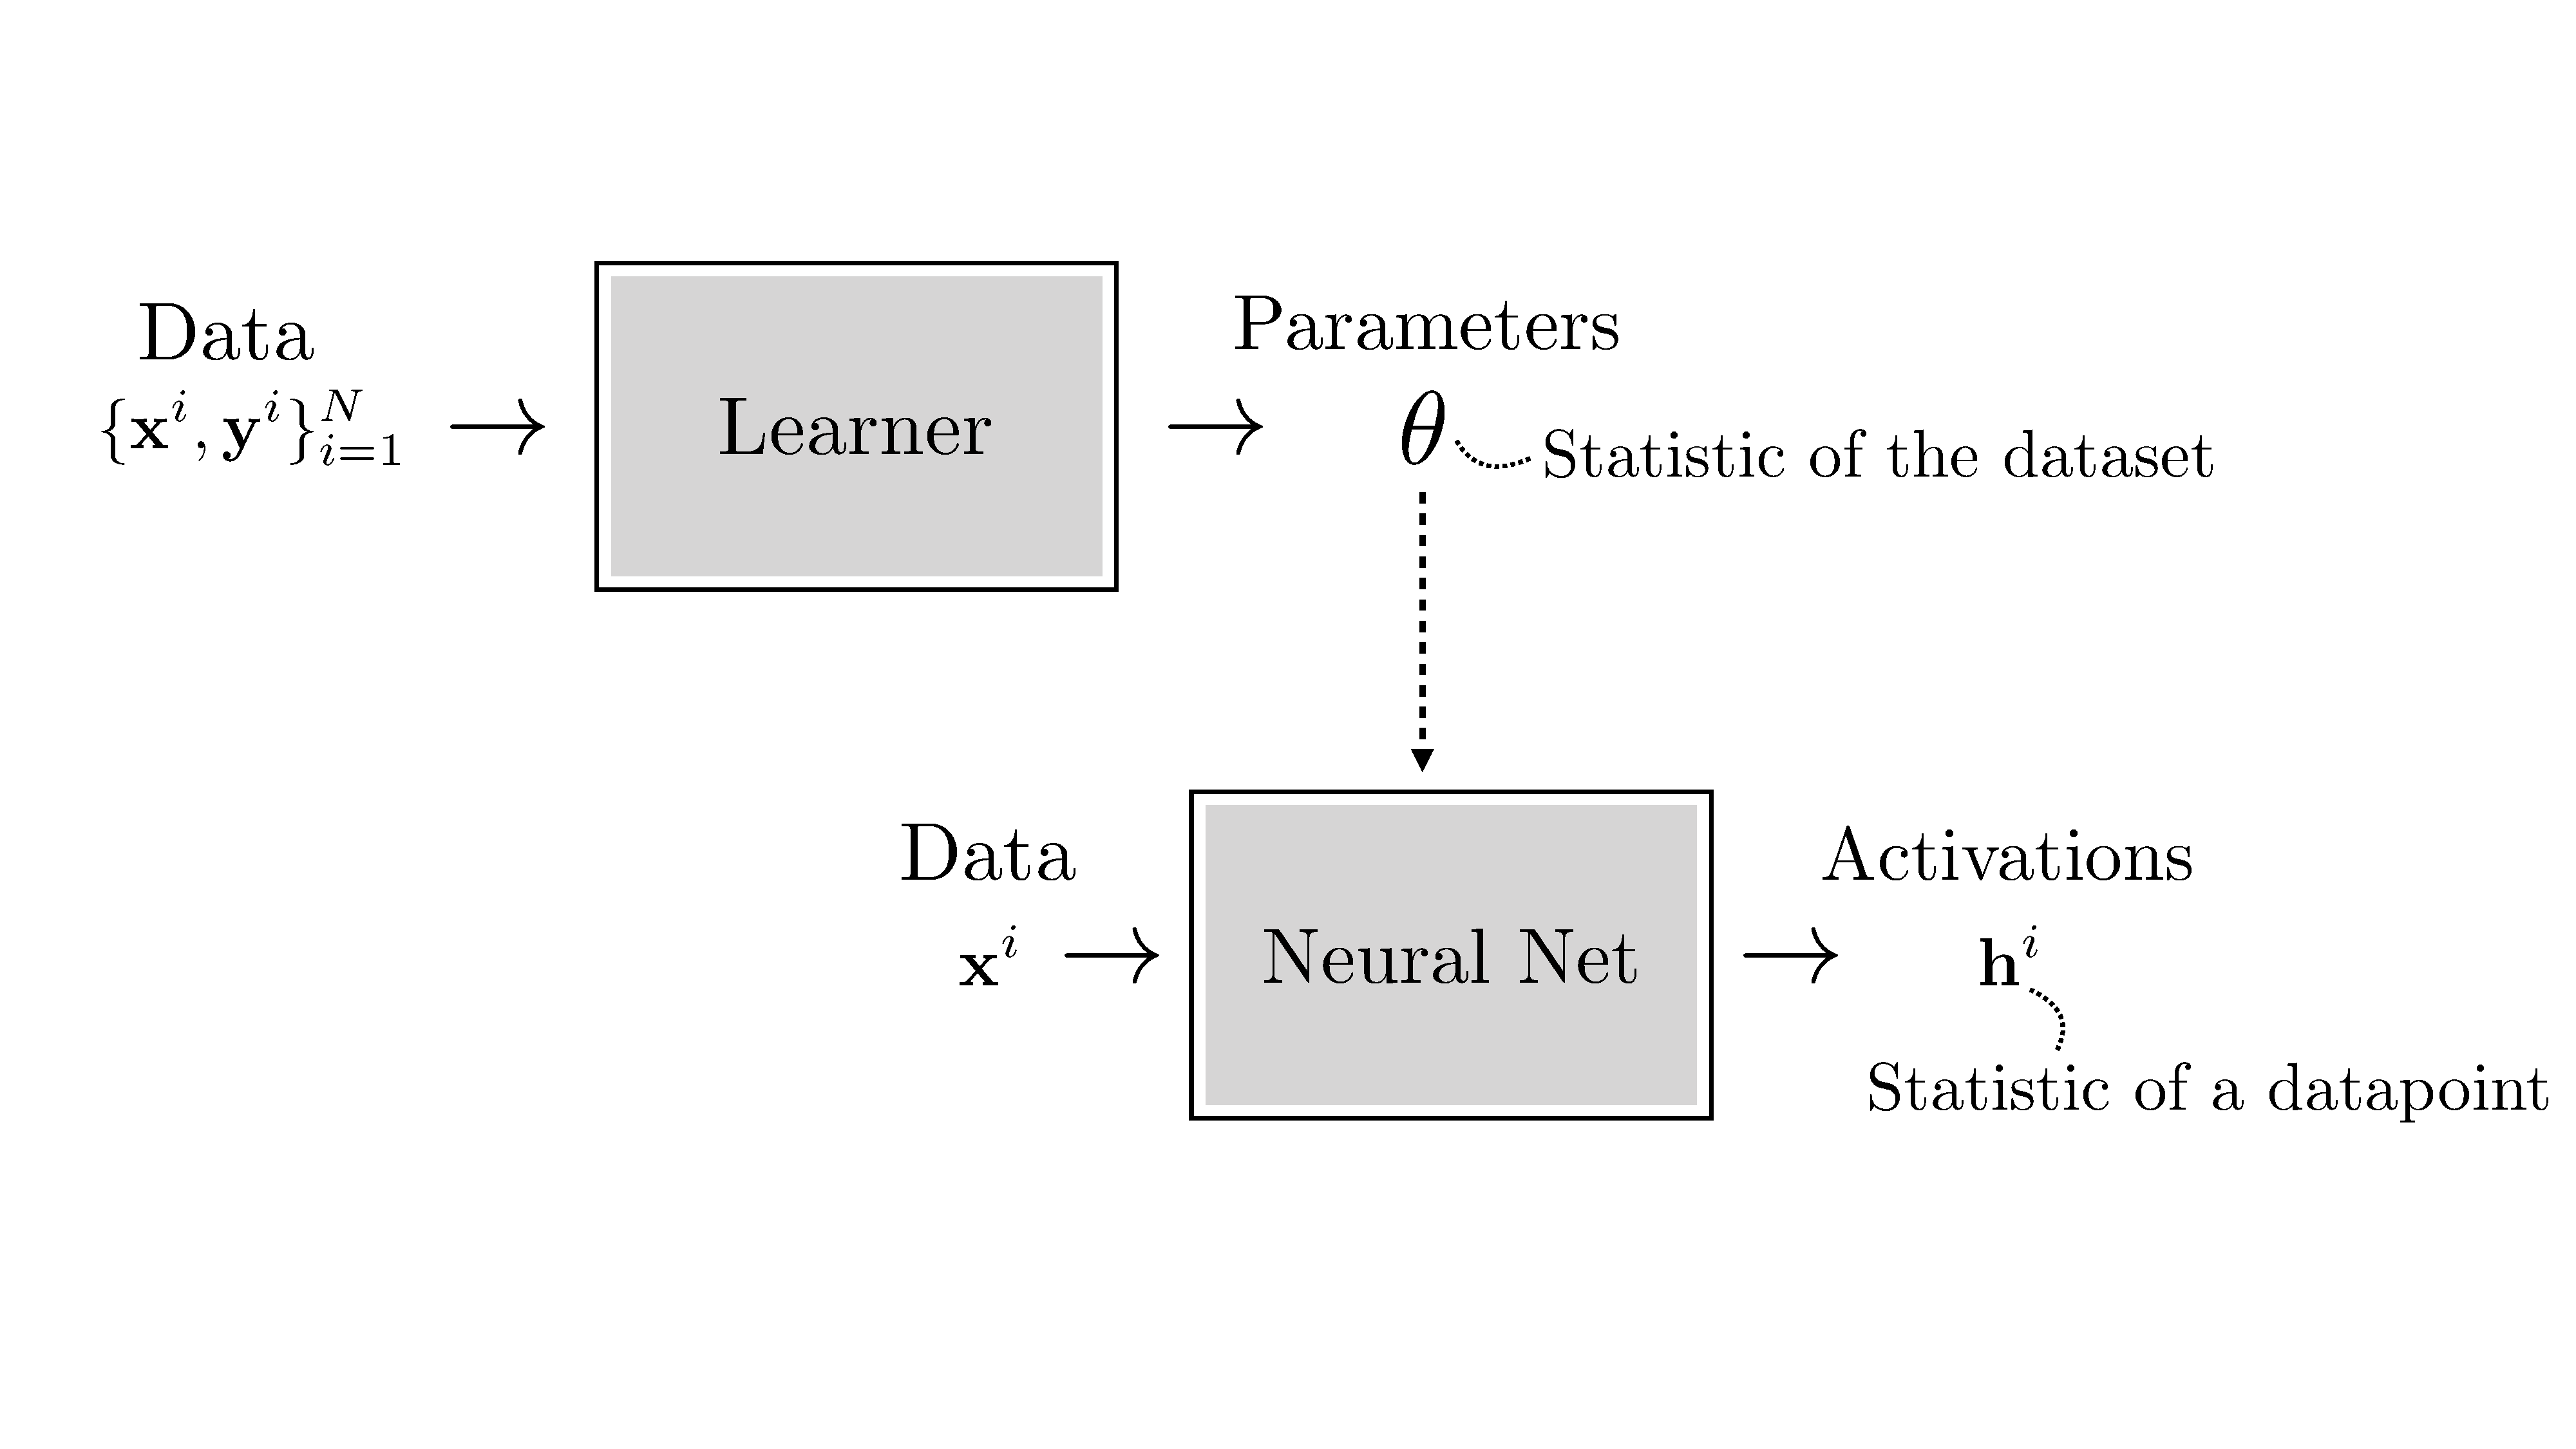
\includegraphics[width=0.7\linewidth]{figures/neural_nets/params_vs_activations.pdf}
}
\caption{Learning is a function that maps a dataset to parameters. Inference, through a neural net, is a function that maps a datapoint to activations.}
\label{fig:neural_nets:params_vs_activations}
\end{figure}

\section{Deep Nets}
Deep nets are neural nets that stack the linear-nonlinear motif many times (\fig{\ref{fig:deep_nets}}):
\begin{figure}[h]
    \centerline{
    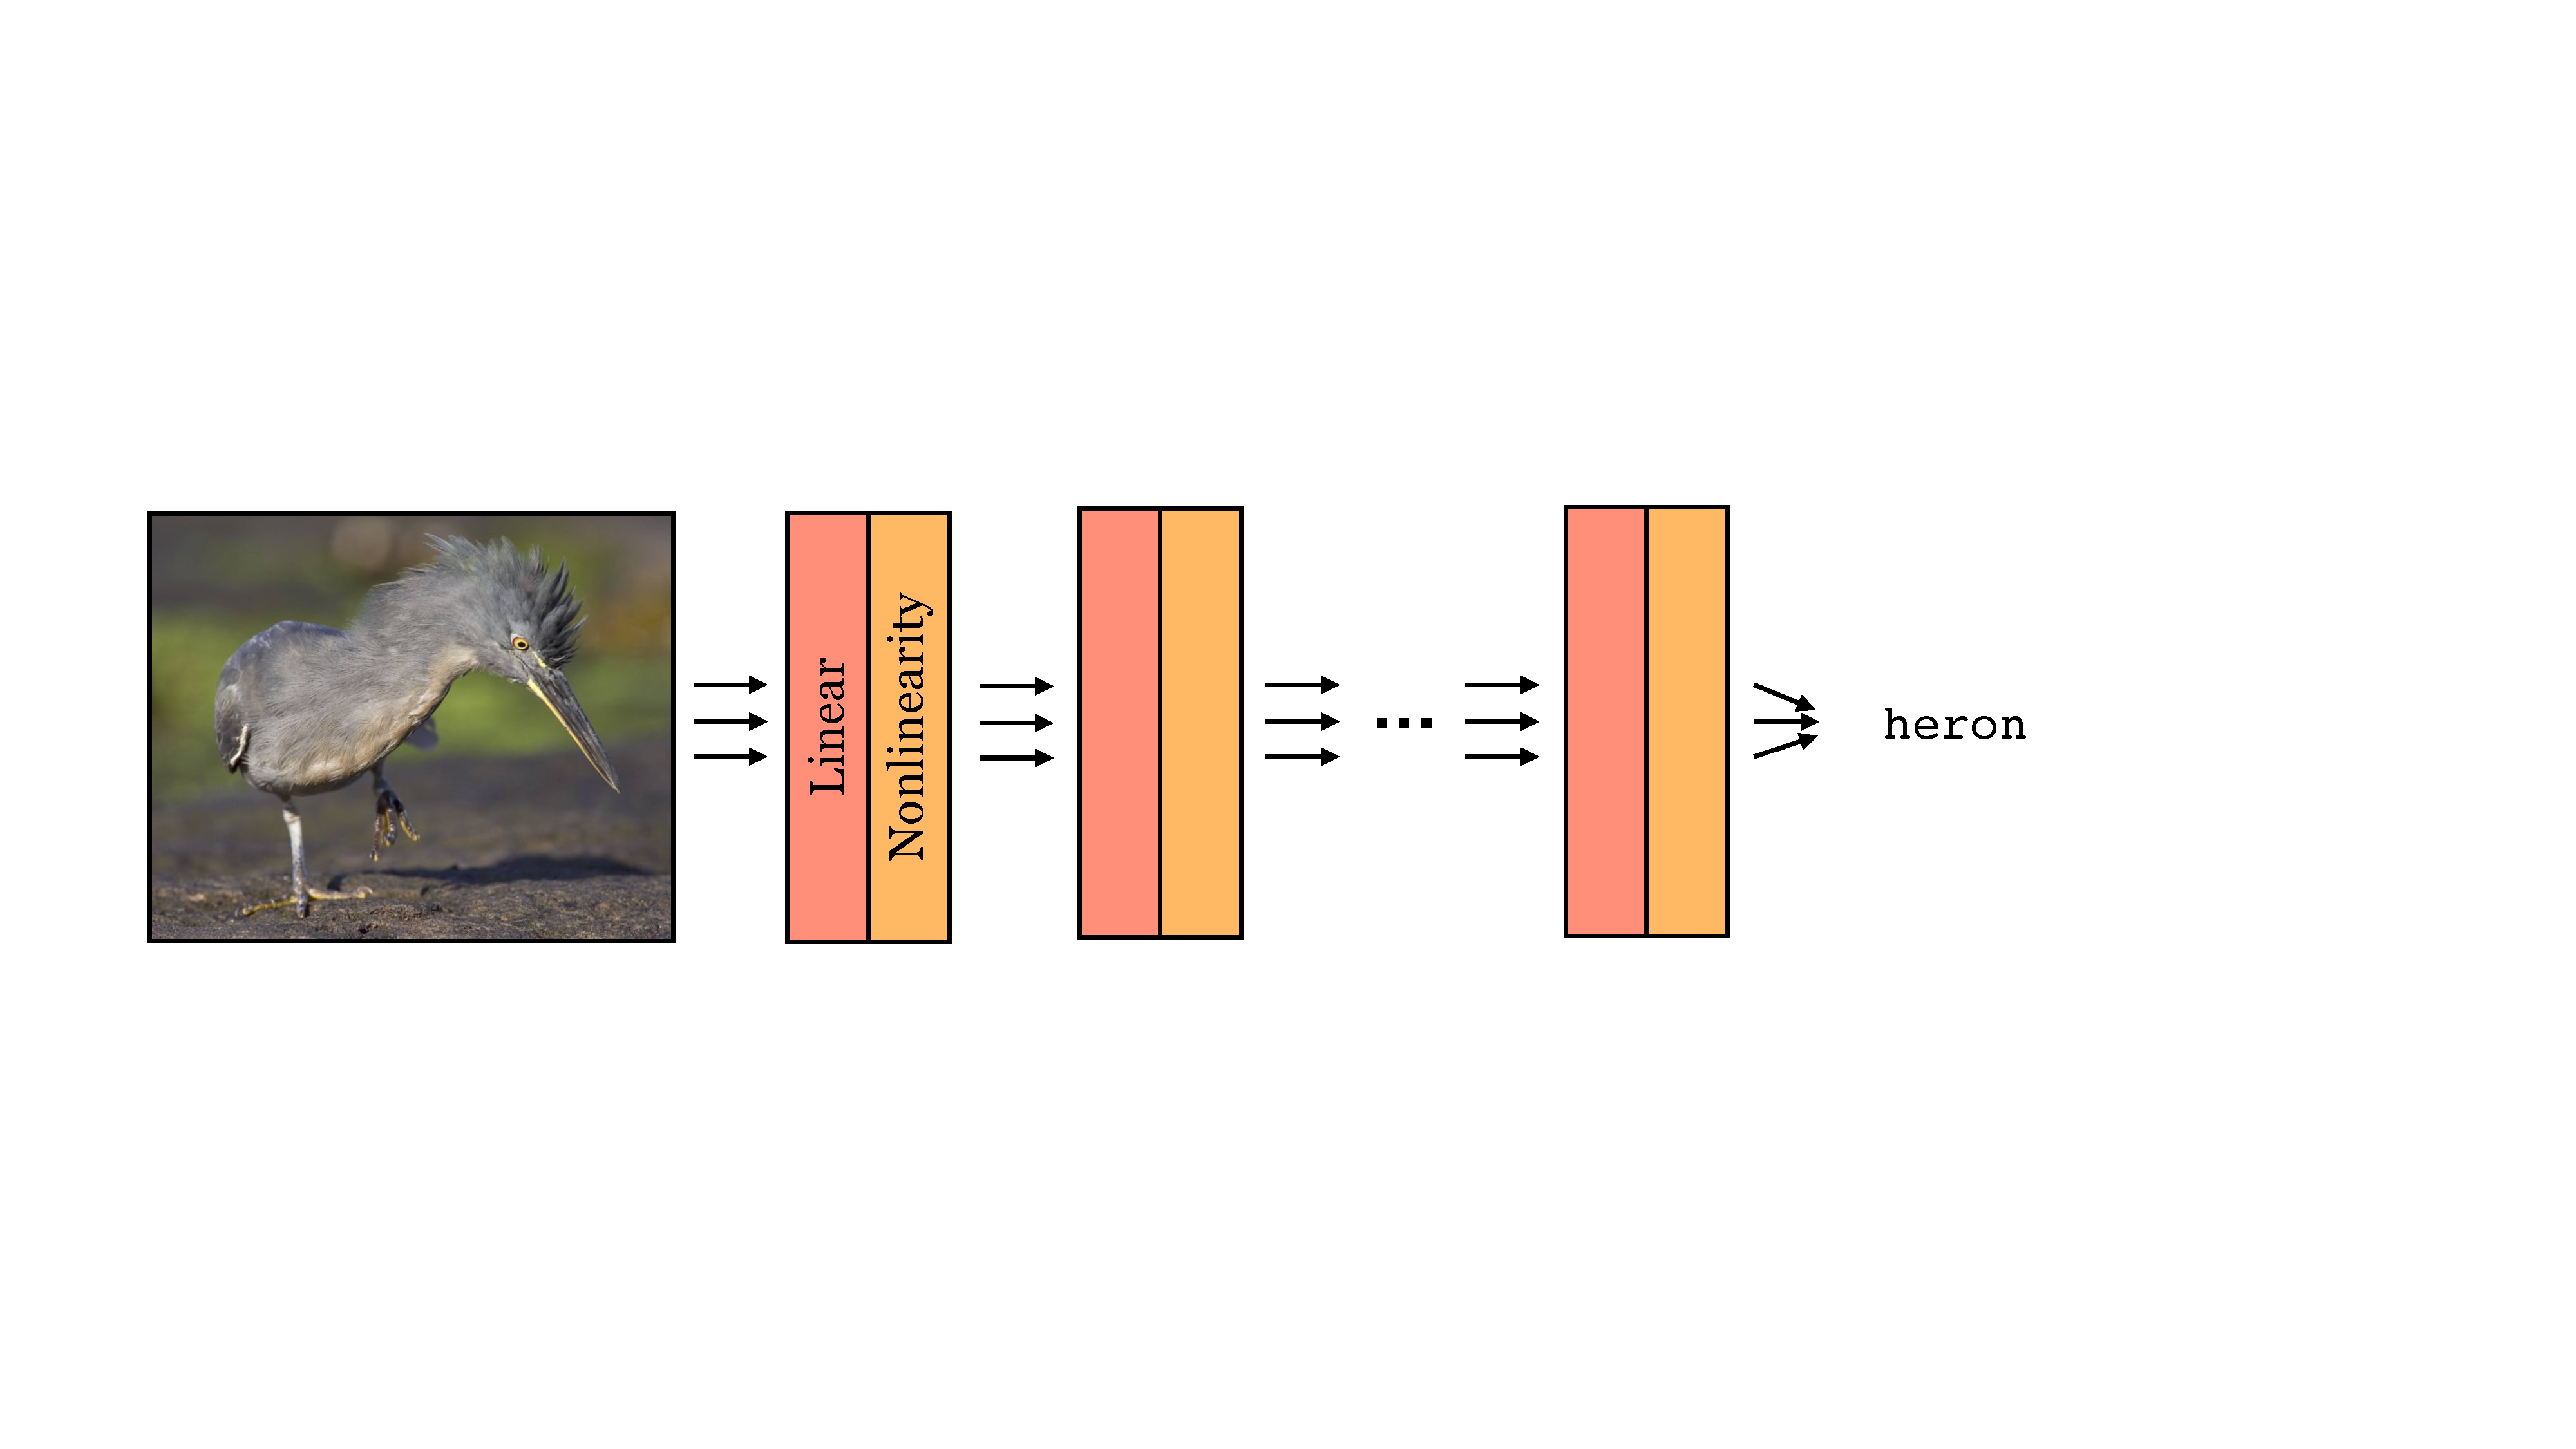
\includegraphics[width=0.65\linewidth]{./figures/neural_nets/deep_nets.pdf}
    }
    \caption{Deep nets consist of linear layers interleaved with nonlinearities.}
    \label{fig:deep_nets}
\end{figure}

Each layer is a function. Therefore, a deep net is a composition of many functions:
\begin{align}
    f(\mathbf{x}) = f_{L}(f_{L-1}(\ldots f_2(f_1(\mathbf{x}))))
\end{align}\marginnote{The $L$ is the number of layers in the net.}[-0.5cm]
These functions are parameterized by weights $[\mathbf{W}_1, \ldots, \mathbf{W}_L]$ and biases $[\mathbf{b}_1, \ldots, \mathbf{b}_L]$. Some layers we will see later have other parameters. Collectively, we will refer to the concatenation of all the parameters in a deep net as $\theta$. %A deep net with the pattern above, that simply alternates linear layers with pointwise non-linearities is called a {\bf multi-layer perceptron}, or {\bf MLP}, as it is can be considered as a set of perceptrons stacked in sequence.

Deep nets are powerful because they can perform nonlinear mappings. In fact, a deep net with sufficiently many neurons can fit almost any desired function arbitrarily closely, a property we will investigate further in \sect{\ref{sec:neural_nets:universal_approximation}}. %The {\bf universal approximation theorem}~\cite{Cybenko1989} states that this is true even for a network with just a single hidden layer. The caveat is that the number of neurons in the hidden layers will have to be very large in order to fit complicated functions. Also, technically, this theorem only holds for continuous functions on compact subsets of $\mathbb{R}^N$ -- for example a neural net cannot fit non-computable functions.


\subsection{Deep Nets Can Perform Nonlinear Classification}

Let's return to our binary classification problem shown previously, but now let's make the two classes not linearly separable. Our new dataset is shown in \fig{\ref{fig:neural_nets:nonseparable_dataset}}.
\begin{figure}[h]
\noindent\hspace{0.3\linewidth}
\begin{minipage}{0.33\linewidth}
\begin{tikzpicture}
\begin{axis}[view={0}{90}, xmin=-1, xmax=1, ymin=-1, ymax=1, 
width=1.0\linewidth, xlabel=$x_1$, ylabel=$x_2$,
align=center,
title={},
axis equal image,
x label style={at={(axis description cs:0.5,-0.17)}},
y label style={at={(axis description cs:-0.17,0.5)}},
%x label style={at={(axis description cs:0.5,0.0)}},
%y label style={at={(axis description cs:0.2,0.5)}},
scatter/classes={%
    pos_correct={mark=text, text mark={\bf 1}},%
    pos_incorrect={mark=text, text mark={\bf \color{red} 1}},%
    neg_correct={mark=text, text mark={\bf 0}},%
    neg_incorrect={mark=text, text mark={\bf \color{red} 0}}}]
%
\addplot[scatter,only marks,%
    scatter src=explicit symbolic]%
table[meta=label] {
x y label
0.1 0.3 neg_correct
0.6 0.15 neg_correct
0.4 0.5 neg_correct
-0.1 0.71 neg_correct
-0.4 0.31 neg_correct
-0.7 0.54 neg_correct
%
0.12 -0.67 pos_correct
-0.34 -0.23 neg_correct
-0.78 -0.68 neg_correct
.84 -0.2 neg_correct
-0.18 -0.5 pos_correct
0.47 -0.64 pos_correct
0.22 -0.28 pos_correct
0.7 -0.54 pos_correct
    };
\end{axis}
\end{tikzpicture}
\end{minipage}
\caption{Dataset that is not linearly separable.}
\label{fig:neural_nets:nonseparable_dataset}
\end{figure}

Here there is no line that can separate the zeros from the ones. Nonetheless, we will demonstrate a multilayer network that can solve this problem. The trick is to just add more layers! We will use the two layer MLP shown in \fig{\ref{fig:neural_nets:simple_MLP_network}}.

\begin{figure}[h]
\centerline{

\noindent\hspace{0.05\linewidth}
\begin{minipage}{.45\linewidth}

\begin{tikzpicture}[>=spaced latex]
\draw [thick] (0,-0.4) circle [radius=0.3] node {$x_2$};
\draw [thick] (0,0.4) circle [radius=0.3] node {$x_1$};
\draw [thick] [nn_edge] (0.3,-0.4) -- (1.0,-0.4);
\draw [thick] [nn_edge] (0.3,0.4) -- (1.0,0.4);
\draw [thick] [nn_edge] (0.3,-0.4) -- (1.0,0.4);
\draw [thick] [nn_edge] (0.3,0.4) -- (1.0,-0.4);
\draw [thick, fill=gray_neuron] (1.3,-0.4) circle [radius=0.3] node {$z_2$};
\draw [thick, fill=gray_neuron] (1.3,0.4) circle [radius=0.3] node {$z_1$};
\draw [thick,dotted] (0.5,-0.9)  .. controls (0.6,-0.75) .. (0.6,-0.6);
\draw (0.6,-1.2) node {$\mathbf{W}_1$};

\draw [thick] [nn_edge] (1.6,-0.4) -- (2.3,-0.4);
\draw [thick] [nn_edge] (1.6,0.4) -- (2.3,0.4);
\draw [thick, fill=gray_neuron] (2.6,-0.4) circle [radius=0.3] node {$h_2$};
\draw [thick, fill=gray_neuron] (2.6,0.4) circle [radius=0.3] node {$h_1$};
\draw [thick,dotted] (3.2,-0.9)  .. controls (3.3,-0.75) .. (3.3,-0.6);
\draw (3.3,-1.2) node {$\mathbf{W}_2$};

\draw [thick] [nn_edge] (2.9,-0.4) -- (3.6,-0.05);
\draw [thick] [nn_edge] (2.9,0.4) -- (3.6,0.05);
\draw [thick, fill=gray_neuron] (3.9,0) circle [radius=0.3] node {$z_3$};
\draw [thick] [nn_edge] (4.2,0) -- (4.9,0);
\draw [thick] (5.2,0) circle [radius=0.3] node {$y$};
\end{tikzpicture}
\caption{A simple MLP network.}
\label{fig:neural_nets:simple_MLP_network}
\end{minipage}
}
\end{figure}

Consider using the following settings for $\mathbf{W}_1$ and $\mathbf{W}_2$:
\begin{align}
    \mathbf{W}_1 = 
        \begin{bmatrix}
            -1 & 1 \\
            1 & 2
        \end{bmatrix}
    ,\quad\quad
    \mathbf{W}_2 = 
        \begin{bmatrix}
            1 & -1
        \end{bmatrix}
\end{align}
The full net then performs the following operation:
\begin{align}
    z_1 &= x_1 - x_2, \quad z_2 = 2x_1 + x_2 &\triangleleft \quad \texttt{linear}\\
    h_1 &= \max(z_1,0), \quad h_2 = \max(z_2,0) &\triangleleft \quad \texttt{relu}\\
    z_3 &= h_1-h_2 &\triangleleft \quad \texttt{linear}\\
    y &= \mathbbm{1}(z_3 > 0) &\triangleleft \quad \text{\texttt{threshold}}
\end{align}
\marginnote{The $\mathbbm{1}$ is the indicator function, which we define as: \begin{equation*}
    \mathbbm{1}(x) = \begin{cases}
                1 & \text{if $x$ is true} \\
                0 & \text{otherwise}
             \end{cases}
\end{equation*}}[-0.5cm]
Here we have introduced a new pointwise nonlinearity, the \index{Rectified linear unit}\textbf{Rectified linear unit} (\textbf{relu}), which is like a graded version of a threshold function, and has the advantage that it yields non-zero gradients over half its domain, thus being amenable to gradient-based learning.

We visualize the values that the neurons take on as a function of $x_1$ and $x_2$ in \fig{\ref{fig:neural_nets:simple_MLP_network_values}}.

\begin{figure}[h]
%\noindent\hspace{0.05\linewidth}
\begin{minipage}{1.0\linewidth}
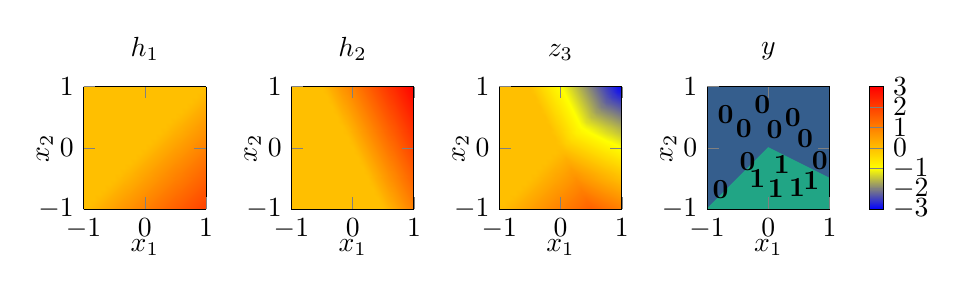
\begin{tikzpicture}
\begin{axis}[name=plot1, view={0}{90}, xmin=-1, xmax=1, ymin=-1, ymax=1, 
width=0.3\linewidth, xlabel=$x_1$, ylabel=$x_2$, 
title=$h_1$,
axis equal image,
x label style={at={(axis description cs:0.5,-0.17)}},
y label style={at={(axis description cs:-0.17,0.5)}},
point meta min=-3, point meta max=3
]
	\addplot3[surf, shader=interp, domain=-1:1] {max(-y+x,0)};
\end{axis}
\begin{axis}[name=plot2, at=(plot1.right of south east), xshift=25, view={0}{90}, xmin=-1, xmax=1, ymin=-1, ymax=1, 
width=0.3\linewidth, xlabel=$x_1$, ylabel=$x_2$, 
title=$h_2$,
axis equal image,
x label style={at={(axis description cs:0.5,-0.17)}},
y label style={at={(axis description cs:-0.17,0.5)}},
point meta min=-3, point meta max=3
]
	\addplot3[surf, shader=interp, domain=-1:1] {max(y+2*x,0)};
\end{axis}
\begin{axis}[name=plot3, at=(plot2.right of south east), xshift=25, view={0}{90}, xmin=-1, xmax=1, ymin=-1, ymax=1, 
width=0.3\linewidth, xlabel=$x_1$, ylabel=$x_2$, 
title=$z_3$,
axis equal image,
x label style={at={(axis description cs:0.5,-0.17)}},
y label style={at={(axis description cs:-0.17,0.5)}},
point meta min=-3, point meta max=3
]
	\addplot3[surf, shader=interp, domain=-1:1] {max(-y+x,0)-max(y+2*x,0)};
\end{axis}
\begin{axis}[name=plot4, at=(plot3.right of south east), xshift=25, view={0}{90}, xmin=-1, xmax=1, ymin=-1, ymax=1, 
width=0.3\linewidth, xlabel=$x_1$, ylabel=$x_2$,
title=$y$,
colorbar,
colorbar style={
        ytick={-3.0,-2.0,-1.0,0,1.0,2.0,3.0},
        yticklabel style={
            align=right
        },
        width=5.0
    },
axis equal image,
x label style={at={(axis description cs:0.5,-0.17)}},
y label style={at={(axis description cs:-0.17,0.5)}},
point meta min=-3, point meta max=3,
%ymajorticks=false
scatter/classes={%
    pos_correct={mark=text, text mark={\bf 1}},%
    pos_incorrect={mark=text, text mark={\bf \color{red} 1}},%
    neg_correct={mark=text, text mark={\bf 0}},%
    neg_incorrect={mark=text, text mark={\bf \color{red} 0}}}]
]
    \addplot3[surf, shader=interp, domain=-1:1] {max(-y+x,0)-max(y+2*x,0)};
	\addplot[fill, index of colormap={5 of viridis}, color=.] coordinates 
		{(-1,-1) (0,0) (1,-0.5) (1,1) (-1,1)} --cycle;
	\addplot[fill, index of colormap={10 of viridis}, color=.] coordinates 
		{(-1,-1) (0,0) (1,-0.5) (1,-1)} --cycle;
    \addplot[scatter,only marks,%
    scatter src=explicit symbolic]%
table[meta=label] {
x y label
0.1 0.3 neg_correct
0.6 0.15 neg_correct
0.4 0.5 neg_correct
-0.1 0.71 neg_correct
-0.4 0.31 neg_correct
-0.7 0.54 neg_correct
%
0.12 -0.67 pos_correct
-0.34 -0.23 neg_correct
-0.78 -0.68 neg_correct
.84 -0.2 neg_correct
-0.18 -0.5 pos_correct
0.47 -0.64 pos_correct
0.22 -0.28 pos_correct
0.7 -0.54 pos_correct
    };
\end{axis}
\end{tikzpicture}
\end{minipage}
\caption{Values of hidden units and output unit for the MLP shown in \fig{\ref{fig:neural_nets:simple_MLP_network}}.}
\label{fig:neural_nets:simple_MLP_network_values}
\end{figure}

As can be seen in the rightmost plot, at the output $y$, this neural net successfully assigns a value of 1 to the region of the dataspace where the datapoints labeled as 1 live. This example demonstrates that is possible to solve nonlinear classification problems with a deep net. In practice, we would want to \textit{learn} the parameter settings that achieve this classification. One way to do so would be to enumerate all possible parameter settings and pick one that successfully separates the zeros from the ones. This kind of exhaustive enumeration is a slow process, but don't worry, in \chap{\ref{chapter:backpropagation}} we will see how to speed things up using gradient descent. But it's worth remarking that enumeration is always a sufficient solution, at least when the possible parameter values form a finite set.


%\subsection{Deep nets can perform nonlinear regression}

%What about regression? It turns out deep nets are good for that too, in fact, they can be effective at implementing many kinds of functional mappings.

%Here are the functions of some random nets:

%\begin{figure}[h]
%    \centering
%    \includegraphics[width=0.19\linewidth]{figures/neural_nets/random_net1.pdf}
%    \includegraphics[width=0.19\linewidth]{figures/neural_nets/random_net2.pdf}
%    \includegraphics[width=0.19\linewidth]{figures/neural_nets/random_net3.pdf}
%    \includegraphics[width=0.19\linewidth]{figures/neural_nets/random_net4.pdf}
%    \includegraphics[width=0.19\linewidth]{figures/neural_nets/random_net5.pdf}
%    \label{fig:random_nets}
%\end{figure}

%Here's what happens as you tune one parameter. You can get it to fit all kinds of things!

\subsection{Deep Nets Are Universal Approximators}\label{sec:neural_nets:universal_approximation}
Not only can deep nets perform nonlinear classification, they can in principle perform \textit{any} continuous input-output mapping. The \index{Universal approximation theorem}{\bf universal approximation theorem}~\cite{Cybenko1989} states that this is true even for a network with just a single hidden layer. The caveat is that the number of neurons in the hidden layers will have to be very large in order to fit complicated functions.\marginnote{Technically, this theorem only holds for continuous functions on compact subsets of $\mathbb{R}^N$ -- for example a neural net cannot fit noncomputable functions. We will not be rigorous in this section. We direct the reader to \cite{TelgarskyNotes2021} for a formal treatment of universal approximation.}[-1.4cm]
%As mentioned above, this is only true if we assume the net can have an arbitrary large number of neurons. In this section we will give an intuition for why this is true.

To get an intuition for why this is true, we will consider the case of approximating an arbitrary function from $\mathbb{R} \rightarrow \mathbb{R}$ with a relu-MLP (an MLP with relu nonlinearities). First observe that any function can be approximated arbitrarily well by a sum of indicator functions, that is, bumps placed at different positions:
\begin{align}
    f(x) \approx \sum_i w_i \mathbbm{1}(\alpha_i < x < \beta_i)\label{eqn:neural_nets:sum_of_indicators}
\end{align}
As an example, in \fig{\ref{fig:neural_nets:curve_as_bump}} we show a curve (blue line) approximated in this way. As the width, $\beta-\alpha$, of the bumps (black lines) goes to zero, the error in the fit goes to zero.
\begin{figure}[h]
    \centerline{
    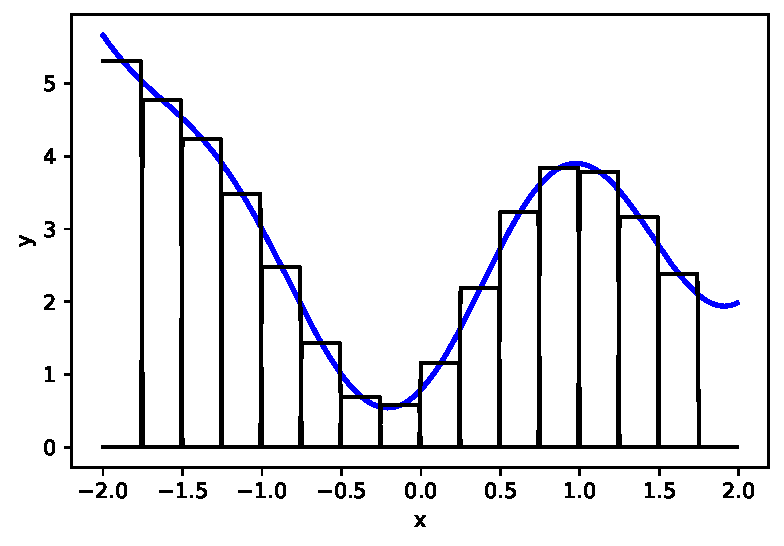
\includegraphics[width=0.35\linewidth]{./figures/neural_nets/curve_as_bumps.pdf}
    }
    \caption{Any function from $\mathbb{R} \rightarrow \mathbb{R}$ can be approximated arbitrarily well by a sum of elementary bumps.}
    \label{fig:neural_nets:curve_as_bump}
\end{figure}

\marginnote{While we only consider scalar functions $\mathbb{R} \rightarrow \mathbb{R}$ here, a similar construction can be used to approximate general functions of the form $\mathbb{R}^n \rightarrow \mathbb{R}^m$.}[-1.8cm]

Next we will show that a relu-MLP can represent \eqn{\ref{eqn:neural_nets:sum_of_indicators}}. The weighted sum $\sum_i w_i \ldots$ is the easy part: that's just a linear layer. So we just have to show that we can also write $\mathbbm{1}(\alpha < x < \beta)$ using linear and relu layers. It turns out the construction is rather simple:
\begin{align}
\mathbbm{1}(\alpha < x < \beta) \approx \texttt{relu}\bigg(\frac{x-(\alpha-\gamma)}{\gamma}\bigg) - \texttt{relu}\bigg(\frac{x-\alpha}{\gamma}\bigg) - \texttt{relu}\bigg(\frac{x-(\beta-\gamma)}{\gamma}\bigg) + \texttt{relu}\bigg(\frac{x-\beta)}{\gamma}\bigg) \label{eqn:neural_nets:bump_as_relu_net}
\end{align}
\marginnote{Here we show how a neural net can represent a function as a sum of basis functions. This idea is also foundational in signal processing, where signals are often represented as a sum of sine waves (\chap{\ref{chapter:fourier_analysis}}), boxes (\fig{\ref{fig:upsampling_and_downsampling:nn_interp}}), or trapezoids (\fig{\ref{fig:bilinear_interp}}).}[-2.0cm]
As $\gamma \rightarrow 0$, this approximation becomes exact. The input to each of the four relus in \eqn{\ref{eqn:neural_nets:bump_as_relu_net}} is an affine function of the input $x$, hence these four values can be represented by a linear layer with four outputs. Then we apply a relu layer to these four values, and finally we apply a linear layer to compute the sum over these relus (a weighted sum with weights [1,-1,-1,1]). Therefore \eqn{\ref{eqn:neural_nets:bump_as_relu_net}} can be implemented as a \texttt{linear}-\texttt{relu}-\texttt{linear} network. In \fig{\ref{fig:neural_nets:bump_as_relus}}, we show an example of constructing a bump in this way.
\begin{figure}[h]
    \centerline{
    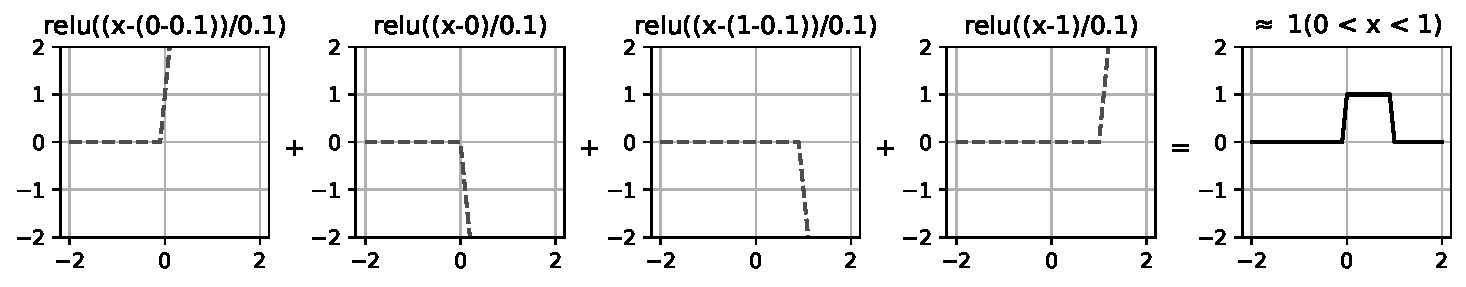
\includegraphics[width=1.0\linewidth]{./figures/neural_nets/bump_as_relus.pdf}
    }
    \caption{A bump can be represented as a weighted sum of shifted and scaled relu functions.}
    \label{fig:neural_nets:bump_as_relus}
\end{figure}

Putting everything together, we have a \texttt{linear}-\texttt{relu}-\texttt{linear} for each bump, followed by a linear layer for summing up all the bumps. The two linear layers in sequence can be collapsed to a single linear layer, and hence the full function can therefore be approximated, to arbitrary precision, by a \texttt{linear}-\texttt{relu}-\texttt{linear} net.\marginnote{Most literature refers to such a net as having a single hidden layer, using the convention that we don't count pre- and postactivation neurons as separate layers.}

%The inputs to each of these $\texttt{relu}$ functions can be implemented as a linear layer (a scaling + bias), so the whole network that approximates a function as a sum of bumps is simply a linear-relu-linear net, i.e. a net with a single hidden layer. 

Notice that in this approximation, we need four relu neurons for each bump we are modeling. Therefore if we want to approximate a very bumpy function, say with $N$ bumps, we will need $4N$ relu neurons. In general, to achieve arbitrarily good approximation to a curve we may need an unbounded number of neurons in our network.

\subsection{Depth versus Width}
Above we saw that if you have a hidden layer with $N$ neurons, you can fit a scalar function with $\mathcal{O}(N)$ bumps. The number of neurons on a single hidden layer is called its \index{Network width}\textbf{width}.\marginnote{If different layers have different numbers of neurons, then we may specify the width per layer. Here we will assume all layers have the same width and simply speak of the width of the network.}[-0.4cm] So, as we increase the width of a network, we can fit ever more complicated functions. What if we instead increase the \index{Network depth}\textbf{depth} of a network, that is, its number of layers? It turns out that this can also be an effective way to increase the capacity of the net, but its effect is a bit different than increasing width.

Interestingly, it is sometimes the case that \textit{deep} nets require far fewer parameters to fit data than \textit{wide} nets. Evidence for this statement comes mostly from empiricism, where researchers have found that deeper nets just work better in practice on many popular problems. However, there is also the beginning of a mathematical theory of when and why this can happen. The basic idea of this theory is to establish that there are certain classes of function that can be represented with a polynomial number of neurons in a depth $d$ network but require an exponential number of neurons in a depth $d^\prime$ network, for certain $d^\prime < d$. Arguments along these lines are called \textbf{depth separations}, and the interested reader can refer to \cite{telgarsky2016benefits} to learn more about this ongoing line of research.

%The above argument shows that relu networks can approximate any function. There is a great deal of additional theory on exactly how many units and layers are needed to approximate exactly what kind of functions to exactly what degree of precision. One important result in this direction is Barron's theorem~\cite{barron1993universal}.

%Chapter \ref{chapter:intro_to_learning}
\section{Deep Learning: Learning with Neural Nets}
Using the formalism we defined in \chap{\ref{chapter:intro_to_learning}}, learning consists of using an \emph{optimizer} to find a function in a \emph{hypothesis space}, that maximizes an \emph{objective}. From this perspective, neural nets are simply a special kind of hypothesis space (and a particular parameterization of that hypothesis space). \index{Deep learning}\textbf{Deep learning} refers to learning algorithms that use this parameterized hypothesis space.

Deep learning also typically involves using gradient-based optimization to search the hypothesis space for the best fit to the data. We will investigate this approach in detail in \chap{\ref{chapter:backpropagation}}, where we will learn about the \textbf{backpropagation} algorithm for gradient-based learning with neural nets. However, it is certainly possible to optimize neural nets with other methods, including zeroth-order optimizers like evolution strategies (\sect{\ref{sec:gradient_descent:zeroth_order}}; \cite{salimans2017evolution}). 

One intriguing alternative to backpropagation is called \index{Hebbian learning}\textbf{Hebbian learning}~\cite{hebb2005organization}. Backpropagation is a \textit{top-down} learning algorithm, where errors incurred at the output (top) of the net are propagated backward to inform earlier layers how to update their weights and biases to minimize the loss, which is a form of learning based on \textit{feedback}. Hebbian learning, in contrast, is a \textit{bottom-up} approach, where neurons wire up just based on the \textit{feedforward} pattern of activity in the net. The canonical learning rule in Hebbian methods is \textbf{Hebb's rule}: ``fire together, wire together.'' That is, we increase the weight of the connection between two neurons whenever the two neurons are active at the same time. Although this learning rule is not explicitly minimizing a loss function, it has been shown to lead to effective neural representations. For example, Hebb-like rules can learn \textbf{infomax} representations, which capture, in the neural activations, as much information as possible about the input signal~\cite{linsker1988self}. Similar rules lead to networks that act like memory banks~\cite{hopfield1982neural}. Hebbian learning is also of interest because it is considered to be more biologically plausible than backpropagation. This is because Hebb's rule can be computed \textit{locally}—each neuron strengthens and weakens its weights based just on the activity of adjacent neurons—whereas backpropagation requires global coordination throughout the neural network. It is currently unknown how this global coordination can be achieved in biological brains.

%Indeed, it is not clear if biological neural nets actually use backpropagation. 

%Alternative optimizers include genetic algorithms~\cite{XX}, simulated annealing~\cite{XX}, and various other kinds of ``random search"~\cite{XX}.

%There is also a broad literature on ``bottom up learning rules" that do not explicitly optimize any objective (though they may implicitly). One such rule, called {\bf Hebbian learning}~\cite{hebb2005organization}, is ``fire together, wire together", that is, we increase the weight of the connection between two neurons whenever the two neurons are active at the same time.
%\marginnote{Remember, you can always just enumerate all possible parameter settings, try each, and pick the best --  smarter optimization is only about making this search faster.}

%\subsection{Classification with a deep net}
%We will now work through an example.


%\section{Regularization in neural nets}
%Weight decay, dropout


\subsection{Data Structures for Deep Learning: Tensors and Batches}

The main data structure that we will encounter in deep learning is the \index{Tensor}{\bf tensor}, which is just a multidimensional array. This may seem simple, but it's important to get comfortable with the conventions of tensor processing.

In general, everything in deep learning is represented as tensors—the input is one tensor, the activations are tensors, the weights are tensors, the outputs are tensors. If you have data that is not natively represented as a tensor, the first step, before feeding it to a deep net, is to convert it into a tensor format. Most often we use tensor of real numbers, that is, the elements of the tensor are in $\mathbb{R}$.

Suppose we have a dataset $\{\mathbf{x}^{(i)}, \mathbf{y}^{(i)}\}_{i=1}^N$ of images $\mathbf{x}$ and labels $\mathbf{y}$. The tensor way of thinking about such a dataset is as two tensors, $\mathbf{X} \in \mathbb{R}^{N \times C_0 \times H \times W }$ and $\mathbf{Y} \in \mathbb{R}^{N \times K}$. The first dimension of the tensor is the number of elements in our dataset. The remaining dimensions are the dimensionality of the images ($C_0$ color channels by height $H$ by width $W$) and labels ($K$-way classification).

The activations in the network are also tensors. For the MLP networks we have seen so far, the activation tensors have shape $N \times C_{\ell}$, where $C_{\ell}$ is the number of neurons on layer $\ell$, sometimes also called \textbf{channels} in analogy to the color channels of the input image. In later chapters we will encounter other architectures where the activation layers have additional dimensions, for example, in convolutional networks we will see activation layers that are of shape $N \times C_{\ell} \times H_{\ell} \times W_{\ell}$.

One other important concept is \index{Batch processing}{\bf batch processing}. Normally, we don't process one image at a time through a neural net. Instead we run a \textit{batch} of images all at once, and they are processed in parallel. A batch sampled from the training data can be denoted as $\{\mathbf{x}_{\texttt{batch}}^{(i)}, \mathbf{y}_{\texttt{batch}}^{(i)}\}_{i=1}^{N_{\texttt{batch}}}$, and the batch represented as a tensor has shape $\mathbf{X} \in \mathbb{R}^{N_{\texttt{batch}} \times C_0 \times H \times W}$ and $\mathbf{Y} \in \mathbb{R}^{N_{\texttt{batch}} \times K}$.

The weights and biases of the net are also usually represented as tensors. The weights and biases of a linear layer will be tensors of shape $\mathbf{W}_{\ell} \in \mathbb{R}^{C_{\ell+1} \times C_{\ell}}$ and $\mathbf{b}_{\ell} \in \mathbb{R}^{C_{\ell+1}}$.

As an example, in \fig{\ref{fig:neural_nets:simple_MLP_network_tensors_and_batches}} below, we visualize all the tensors associated with a batch of three datapoints being processed by the MLP from \fig{\ref{fig:neural_nets:simple_MLP_network}}. For this network, the input is not a set of images but instead a set of vectors $\mathbf{X} \in \mathbb{R}^{N_{\texttt{batch}} \times C_0}$. The output is one value for each input vector, so we have $\mathbf{Y} \in \mathbb{R}^{N_{\texttt{batch}} \times 1}$.

\begin{figure}[h]
\centerline{

\noindent\hspace{0.05\linewidth}
\begin{minipage}{0.65\linewidth}
\begin{tikzpicture}
\draw[step=0.25cm,color=data_color_dark] (0,0) grid (0.5,0.75);
\draw [decorate,decoration={brace,amplitude=5pt}] (-0.1,0) -- (-0.1,0.75) node [black,midway,xshift=-0.7cm] {$N_{\texttt{batch}}$};
\draw [decorate,decoration={brace,mirror,amplitude=5pt}] (0,-0.1) -- (0.5,-0.1) node [black,midway,yshift=-0.5cm] {$C_0$};
\node at (0.25,1.0) {$\mathbf{X}$}; \draw [thick] [nn_edge] (0.6,0.4) -- (1.9,0.4);
\draw[step=0.25cm,color=param_color_dark] (0.99,0.749) grid (1.5,1.25); \node at (1.25,1.7) {$\mathbf{W}_1$};
\draw[step=0.25cm,color=data_color_dark] (1.99,0) grid (2.5,0.75); 
\draw [decorate,decoration={brace,mirror,amplitude=5pt}] (2.0,-0.1) -- (2.5,-0.1) node [black,midway,yshift=-0.5cm] {$C_1$};
\node at (2.25,1.0) {$\mathbf{Z}_1$}; \draw [thick] [nn_edge] (2.6,0.4) -- (2.9,0.4);
\draw[step=0.25cm,color=data_color_dark] (2.99,0) grid (3.5,0.75); 
\draw [decorate,decoration={brace,mirror,amplitude=5pt}] (3.0,-0.1) -- (3.5,-0.1) node [black,midway,yshift=-0.5cm] {$C_1$};
\node at (3.25,1.0) {$\mathbf{H}_1$}; \draw [thick] [nn_edge] (3.6,0.4) -- (4.9,0.4);
\draw[step=0.25cm,color=param_color_dark] (3.99,0.749) grid (4.5,1.0); \node at (4.25,1.5) {$\mathbf{W}_2$};
\draw[step=0.25cm,color=data_color_dark] (4.99,0) grid (5.25,0.75); 
\draw [decorate,decoration={brace,mirror,amplitude=5pt}] (5.0,-0.1) -- (5.25,-0.1) node [black,midway,yshift=-0.5cm] {$C_2$};
\node at (5.125,1.0) {$\mathbf{Z}_2$}; \draw [thick] [nn_edge] (5.4,0.4) -- (5.9,0.4);
\draw[step=0.25cm,color=data_color_dark] (5.99,0) grid (6.25,0.75); 
\draw [decorate,decoration={brace,mirror,amplitude=5pt}] (6.0,-0.1) -- (6.25,-0.1) node [black,midway,yshift=-0.5cm] {$1$};
\node at (6.125,1.0) {$\mathbf{Y}$};
\end{tikzpicture}
\end{minipage}
}
\caption{The tensors that represent one pass through the MLP in \fig{\ref{fig:neural_nets:simple_MLP_network}}.}
\label{fig:neural_nets:simple_MLP_network_tensors_and_batches}
\end{figure}
where the capital letters are the batches of datapoints and activations corresponding to the lowercase names of datapoints and hidden units in \fig{\ref{fig:neural_nets:simple_MLP_network}}.

This example shows the basic concept of working with tensors and batches for one-dimensional data, but, in vision, most of the time we will be working with higher-dimensional tensors. For image data we typically use four-dimensional tensors: batch $\times$ channels $\times$ height $\times$ width; for videos we may use five-dimensional tensors: batch $\times$ channels $\times$ height $\times$ width $\times$ time. Three-dimensional (3D) scans have an additional \textit{depth} spatial dimension; videos of 3D data could therefore be represented by six-dimensional tensors. As you can see, thinking in terms of two-dimensional matrices is not quite sufficient. Instead, you should be imagining data processing as operating on $N$-dimensional tensors, sliced and diced in different ways. As a step in this direction, you may find it useful to visualize tensors in 3D, as shown in \fig{\ref{fig:neural_nets:3D_tensor_example}}.
\begin{figure}[h]
\centerline{
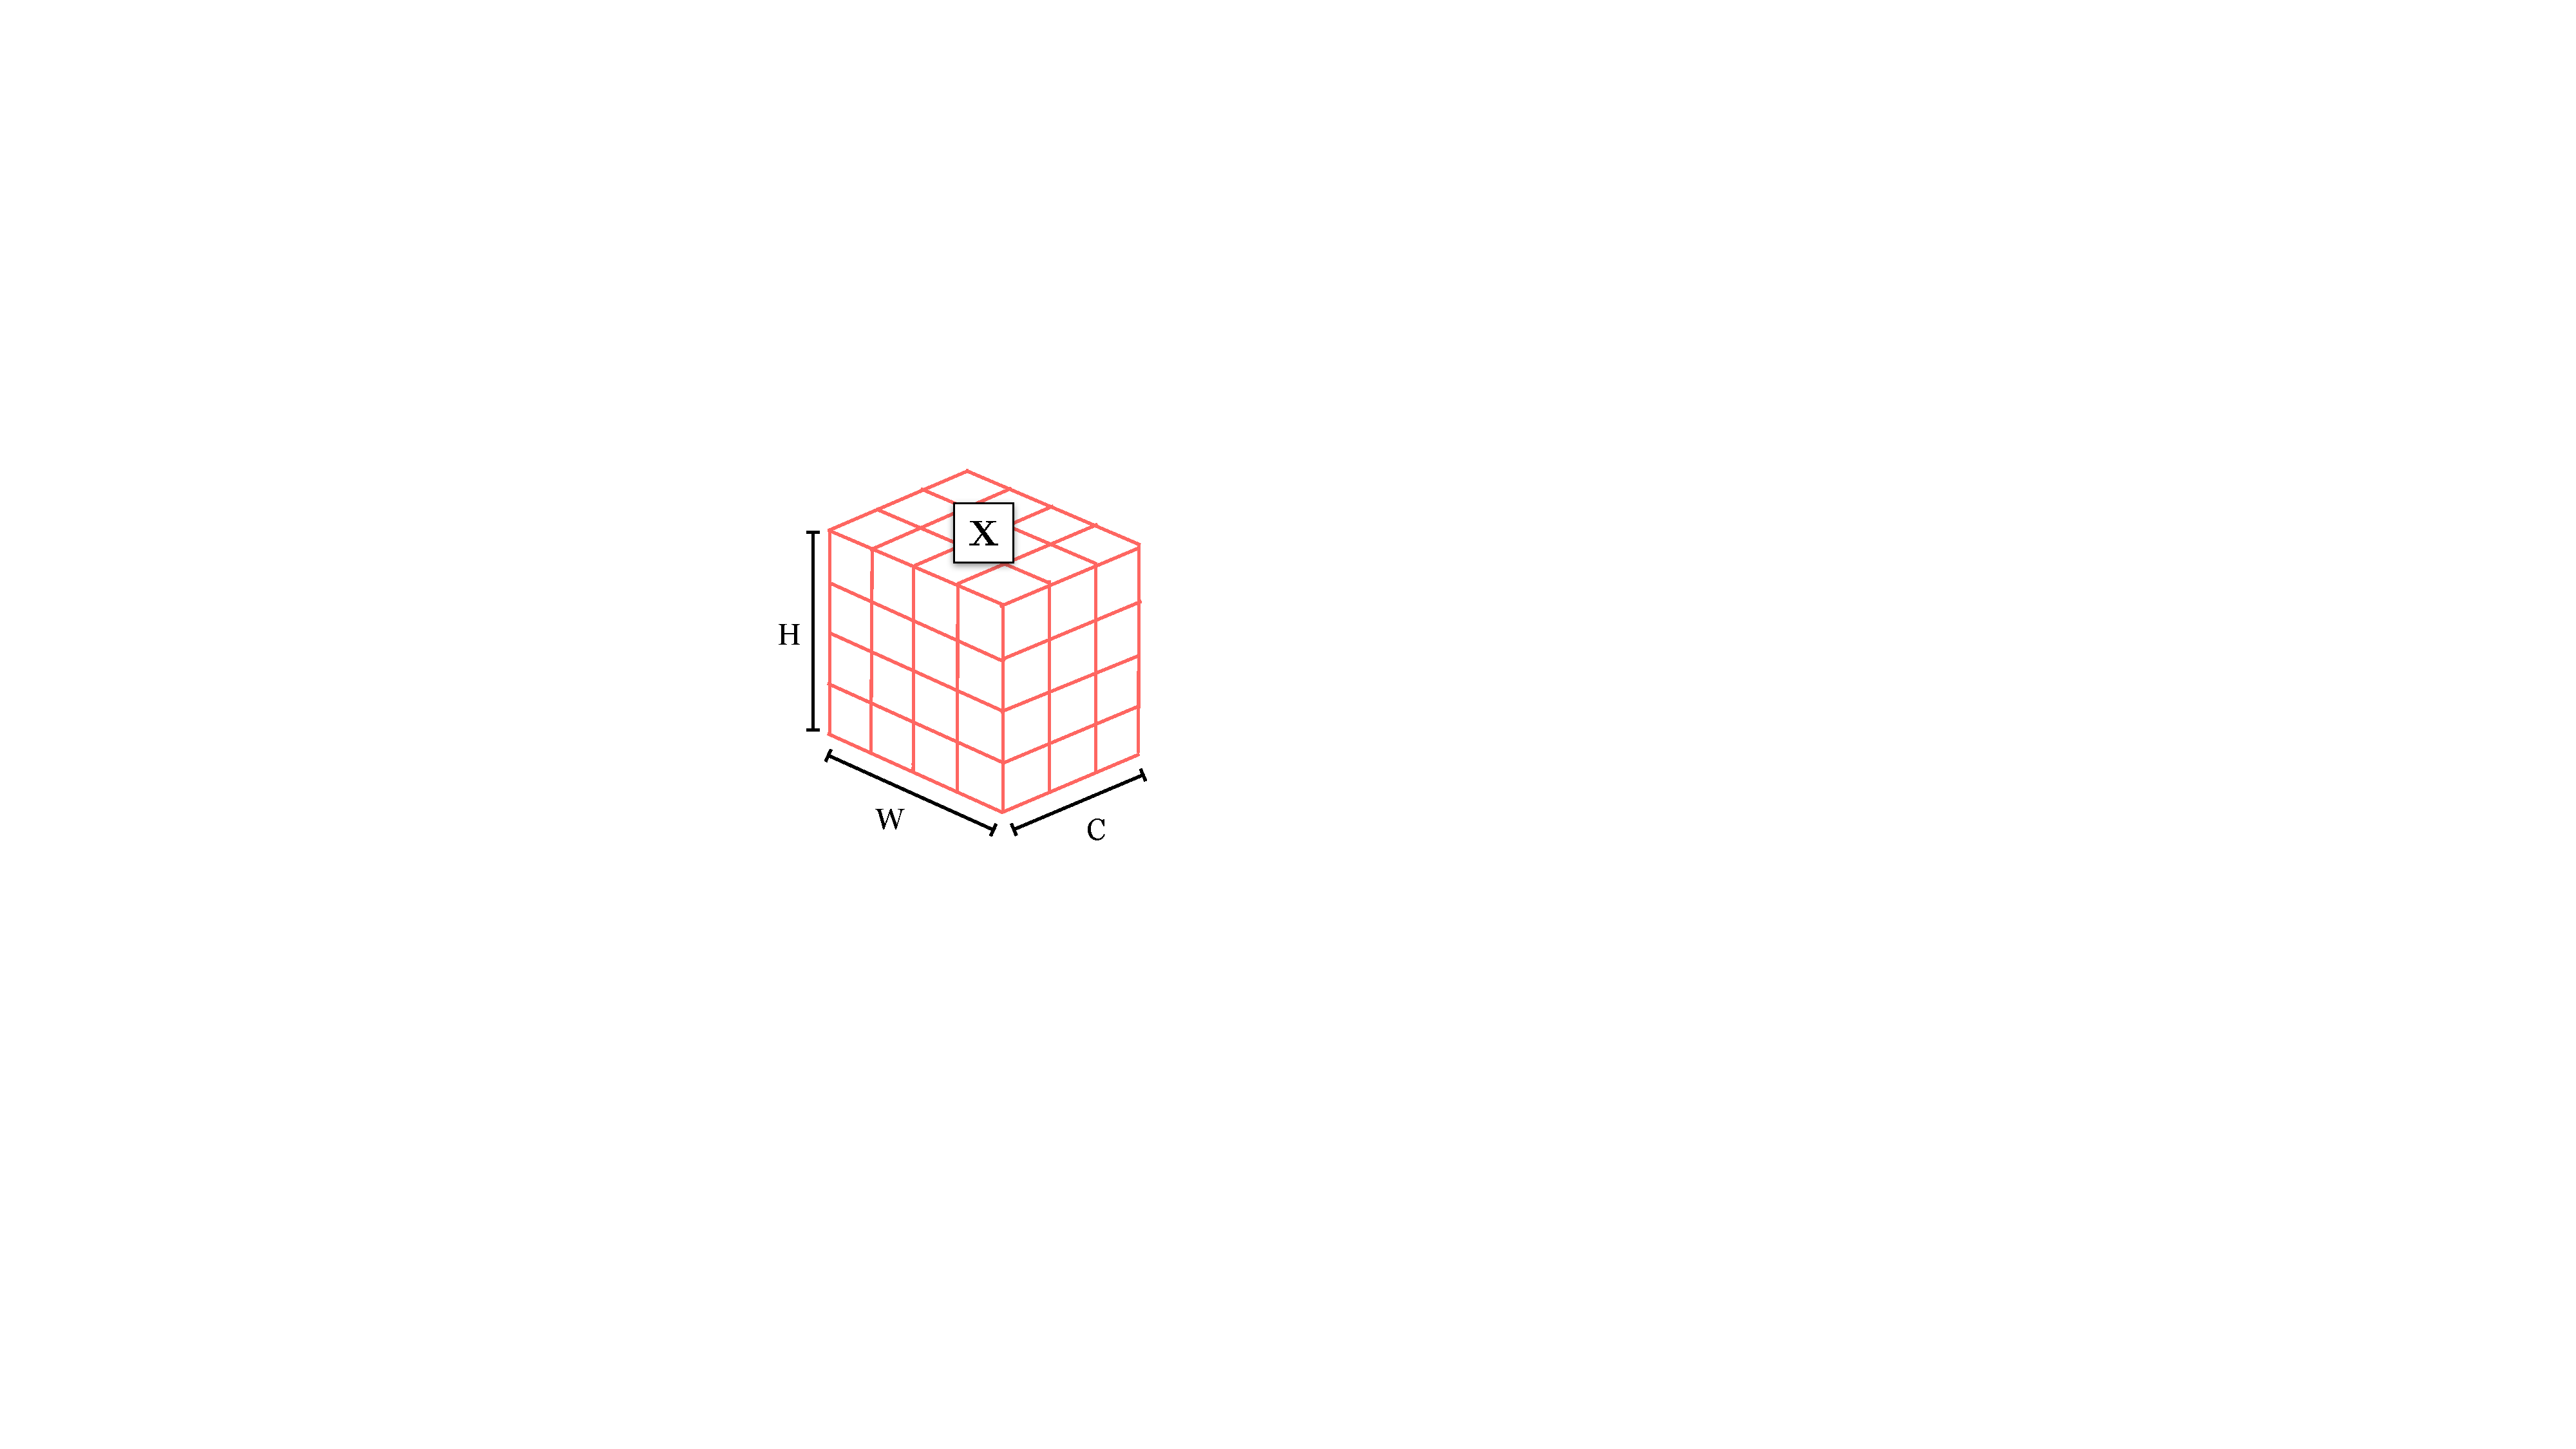
\includegraphics[width=0.2\linewidth]{figures/neural_nets/3D_tensor_example.pdf}
}
\caption{A 3D tensor that could represent an $C \times H \times W$ color image.}
\label{fig:neural_nets:3D_tensor_example}
\end{figure}

This is closer to the actual ND tensors vision systems work with, and many concepts can be adequately captured just by thinking in 3D. We will see some examples in later chapters.

% \subsection{Batch learning}
% To train a deep net we run a batch of data through it, and then compute the loss summed (or averaged) across the batch. This scores how good the current parameter settings of the network are, as estimated on a batch of training data. We can then update the parameters (e.g., at random, or with gradient descent, which we will see in the next chapter) and try again to get a better score on the next data batch. The computational pipeline, visualized as data tensors being transformed layer by layer, looks like this:

% \noindent\hspace{0.05\linewidth}
% \begin{minipage}{0.75\linewidth}
% \begin{tikzpicture}
% \draw[step=0.25cm,color=data_color] (0,3.99) grid (0.5,4.75); \node at (0.25,5.0) {$\mathbf{X}$}; \draw [thick] [nn_edge] (0.6,4.4) -- (1.9,4.4);
% \draw[step=0.25cm,color=data_color] (1.99,3.99) grid (2.5,4.75); \node at (2.25,5.0) {$\mathbf{Z}_1$}; \draw [thick] [nn_edge] (2.6,4.4) -- (2.9,4.4);
% \draw[step=0.25cm,color=data_color] (2.99,3.99) grid (3.5,4.75); \node at (3.25,5.0) {$\mathbf{H}_1$}; \draw [thick] [nn_edge] (3.6,4.4) -- (4.9,4.4);
% \draw[step=0.25cm,color=data_color] (4.99,3.99) grid (5.25,4.75); \node at (5.125,5.0) {$\mathbf{Z}_2$}; \draw [thick] [nn_edge] (5.4,4.4) -- (5.9,4.4);
% \draw[step=0.25cm,color=data_color] (5.99,3.99) grid (6.25,4.75); \node at (6.125,5.0) {$\mathbf{Y}$};
% %
% \draw[step=0.25cm,color=data_color] (0,1.99) grid (0.5,2.75); \node at (0.25,3.0) {$\mathbf{X}$}; \draw [thick] [nn_edge] (0.6,2.4) -- (1.9,2.4);
% \draw[step=0.25cm,color=data_color] (1.99,1.99) grid (2.5,2.75); \node at (2.25,3.0) {$\mathbf{Z}_1$}; \draw [thick] [nn_edge] (2.6,2.4) -- (2.9,2.4);
% \draw[step=0.25cm,color=data_color] (2.99,1.99) grid (3.5,2.75); \node at (3.25,3.0) {$\mathbf{H}_1$}; \draw [thick] [nn_edge] (3.6,2.4) -- (4.9,2.4);
% \draw[step=0.25cm,color=data_color] (4.99,1.99) grid (5.25,2.75); \node at (5.125,3.0) {$\mathbf{Z}_2$}; \draw [thick] [nn_edge] (5.4,2.4) -- (5.9,2.4);
% \draw[step=0.25cm,color=data_color] (5.99,1.99) grid (6.25,2.75); \node at (6.125,3.0) {$\mathbf{Y}$};
% %
% \draw[step=0.25cm,color=data_color] (0,0) grid (0.5,0.75); \node at (0.25,1.0) {$\mathbf{X}$}; \draw [thick] [nn_edge] (0.6,0.4) -- (1.9,0.4);
% \draw[step=0.25cm,color=data_color] (1.99,0) grid (2.5,0.75); \node at (2.25,1.0) {$\mathbf{Z}_1$}; \draw [thick] [nn_edge] (2.6,0.4) -- (2.9,0.4);
% \draw[step=0.25cm,color=data_color] (2.99,0) grid (3.5,0.75); \node at (3.25,1.0) {$\mathbf{H}_1$}; \draw [thick] [nn_edge] (3.6,0.4) -- (4.9,0.4);
% \draw[step=0.25cm,color=data_color] (4.99,0) grid (5.25,0.75); \node at (5.125,1.0) {$\mathbf{Z}_2$}; \draw [thick] [nn_edge] (5.4,0.4) -- (5.9,0.4);
% \draw[step=0.25cm,color=data_color] (5.99,0) grid (6.25,0.75); \node at (6.125,1.0) {$\mathbf{Y}$};
% \end{tikzpicture}
% \end{minipage}


\section{Catalog of Layers}
Below, we use the color blue to denote \textcolor{param_color_dark}{\bf parameters} and the color red to denote \textcolor{data_color_dark}{\bf data/activations} (inputs and outputs to each layer).
\marginnote{We color equations in this way only in this chapter, to make clear the roles of different variables. However, be on the lookout for these colors in figures later in the book. We will often draw activations in red and parameters in blue.}[-0.4cm]

\subsection{Linear Layers}
Linear layers are the workhorses of deep nets. Almost all parameters of the network are contained in these layers; we call these parameters the weights and biases. We have already introduced linear layers previously. They look like this:
\begin{align}
    \textcolor{data_color_dark}{\xout} = \textcolor{param_color_dark}{\mathbf{W}} \textcolor{data_color_dark}{\xin} + \textcolor{param_color_dark}{\mathbf{b}} & \quad\quad \triangleleft \quad\texttt{linear}
\end{align}

\subsection{Activation Layers}

\begin{figure}[t]
    \centerline{
    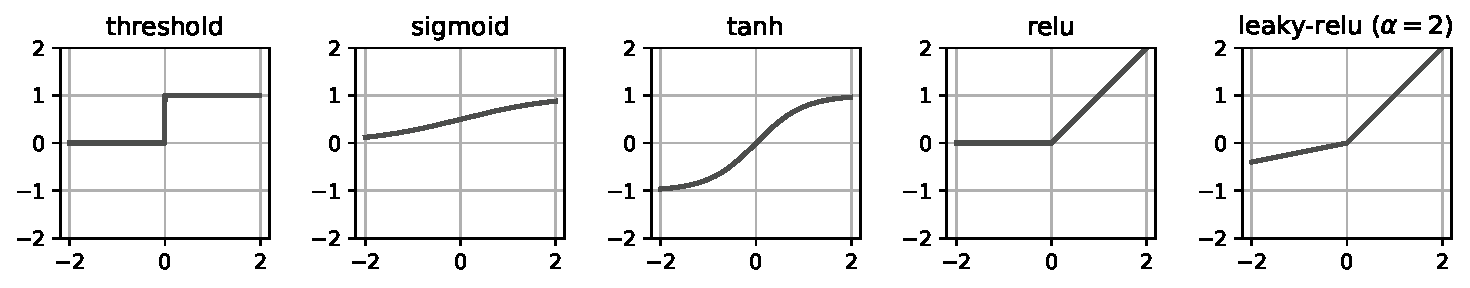
\includegraphics[width=1.0\linewidth]{./figures/neural_nets/pointwise_nonlinearities.pdf}
    }
    \caption{Common pointwise nonlinearities.}
    \label{fig:neural_nets:pointwise_nonlinearities}
\end{figure}

If a net only contained linear layers then it could only compute linear functions. This is because the composition of $N$ linear functions is a linear function. \index{Activation function}\textbf{Activation layers} add nonlinearity. Activation layers are typically pointwise functions, applying a scalar to scalar mapping on each dimension of the input vector. Typically parameters of these layers, if any, are not learned (but they can be). Some common activation layers are defined below and are plotted in \fig{\ref{fig:neural_nets:pointwise_nonlinearities}}:
\begin{align}
    \textcolor{data_color_dark}{\xoutindexed}[i] &= 
        \begin{cases}
            1, &\text{if} \quad \textcolor{data_color_dark}{\xinindexed}[i] > 0\\
            0,              & \text{otherwise}
        \end{cases} & \quad\quad \triangleleft \quad \texttt{threshold}\\
    \textcolor{data_color_dark}{\xoutindexed}[i] &= \frac{1}{1 + e^{-\textcolor{data_color_dark}{\xinindexed}[i]}} & \quad\quad \triangleleft \quad \texttt{sigmoid}\\
    \textcolor{data_color_dark}{\xoutindexed}[i] &= 2*\texttt{sigmoid}(2*\textcolor{data_color_dark}{\xinindexed}[i])-1 & \quad\quad \triangleleft \quad \texttt{tanh}\\
    \textcolor{data_color_dark}{\xoutindexed}[i] &= \max(\textcolor{data_color_dark}{\xinindexed}[i],0) & \quad\quad \triangleleft \quad \texttt{relu}\\
    \textcolor{data_color_dark}{\xoutindexed}[i] &= 
        \begin{cases}
            \max(\textcolor{data_color_dark}{\xinindexed}[i],0), &\text{if} \quad \textcolor{data_color_dark}{\xinindexed}[i] \geq 0\\
            \textcolor{param_color_dark}{a}\min(\textcolor{data_color_dark}{\xinindexed}[i],0),              & \text{otherwise}
        \end{cases} & \quad\quad \triangleleft \quad \texttt{leaky-relu}
\end{align}

\subsection{Normalization Layers}\label{sec:neural_nets:normalization_layers}
\index{Normalization layers}
Normalization layers add another kind of nonlinearity. Instead of being a pointwise nonlinearity, like in activation layers, they are nonlinearities that perturb each neuron based on the collective behavior of a set of neurons. Let's start with the example of \index{Batch normalization}{\bf batch normalization} (\textbf{batchnorm})~\cite{ioffe2015batch}.

Batchnorm {\bf standardizes} each neural activation with respect to its mean and variance over a batch of datapoints. Mathematically, 
\begin{align}
    \textcolor{data_color_dark}{\xoutindexed}[i] = \textcolor{param_color_dark}{\gamma}\frac{\textcolor{data_color_dark}{\xinindexed}[i] - \mathbb{E}[\textcolor{data_color_dark}{\xinindexed}[i]]}{\sqrt{\texttt{Var}[\textcolor{data_color_dark}{\xinindexed}[i]]}} + \textcolor{param_color_dark}{\beta} & \quad\quad \triangleleft \quad \texttt{batchnorm}
\end{align}
\marginnote{Recall from statistics that the standard score of a draw of a random variable is how many standard deviations it differs from the mean: $z = \frac{x-\mu}{\sigma}$.}[-0.4cm]
where $\textcolor{param_color_dark}{\gamma}$ and $\textcolor{param_color_dark}{\beta}$ are learned parameters of this layer that maintain expressivity so that the layer can output values with non-zero mean and non-unit variance. Most commonly batchnorm is applied using training batch statistics to compute the mean and variance, which change batch to batch. At test time, aggregate statistics from the training data are used. However, using test batch statistics can be useful for achieving invariance to changes in the statistics from training data to test data~\cite{wang2020fully}.

There are numerous other normalization layers that have been defined over the years. Two more that we will highlight are \index{$L_2$ normalization}\textbf{$L_2$ normalization} and \index{Layer normalization}\textbf{layer normalization} (\textbf{layernorm})~\cite{ba2016layer}. $L_2$ normalization projects the inputs onto the unit hypersphere, which useful for bounding the activations to unit vectors:
\begin{align}
    \textcolor{data_color_dark}{\xoutindexed}[i] &= \frac{\textcolor{data_color_dark}{\xinindexed}[i]}{\norm{\textcolor{data_color_dark}{\xin}}_2} & \quad\quad \triangleleft \quad \texttt{L2-norm}
\end{align}
%This operation projects the inputs onto the unit hypersphere -- quite a nice trick.
Layernorm is similar except that it standardizes the vector of input activations:
\begin{align}
    \mu &= \frac{1}{n} \sum_{i=1}^n \textcolor{data_color_dark}{\xinindexed}[i]\\
    \sigma^2 &= \frac{1}{n} \sum_{i=1}^n (\textcolor{data_color_dark}{\xinindexed}[i] - \mu)^2\\
    \textcolor{data_color_dark}{\xoutindexed}[i] &= \textcolor{param_color_dark}{\gamma}\frac{\textcolor{data_color_dark}{\xinindexed}[i] - \mu}{\sigma} + \textcolor{param_color_dark}{\beta} & \quad\quad \triangleleft \quad \texttt{layernorm}
\end{align}
\marginnote{Notice that layernorm, like $L_2$-normalization, maps the activation vector to the surface of a hypersphere, but it also centers the activations to have zero mean, and then scales and shifts the activations via $\gamma$ and $\beta$. As an exercise, see if you can write layernorm using $L_2$-normalization as one of the steps.}[-3.2cm]
Notice that layernorm also looks quite similar to batchnorm. Both standardize activations but do so with respect to different statistics. Layernorm computes a mean and variance over elements of a datapoint $\xin$, and will do so separately for each such datapoint in a batch. Batchnorm computes the mean and variance per channel over datapoints in a batch. If we have a batch stored in the tensor $\mathbf{X} \in \mathbb{R}^{N_{\texttt{batch}} \times C}$, then what layernorm does looks just like a ``transpose'' of what batchnorm does. Batchnorm standardizes each element of the tensor by the mean and variance of its column. Layernorm standardizes each element by the mean and variance of its row:
\begin{figure}[h!]
    \centerline{
    %\noindent\hspace{0.05\linewidth}
    %\begin{minipage}{0.65\linewidth}
    \begin{tikzpicture}
        \def\Nbatch{5}
        \def\Nchannels{6}
        \def\cellwidth{0.25}
        %
        % draw batchnorm
        \draw[step=\cellwidth,color=data_color_dark,fill=gray!33, thick] (0,0) rectangle ++(1*\cellwidth, -\Nbatch*\cellwidth);
        \draw[step=\cellwidth,color=data_color_dark] (0,0) grid (\Nchannels*\cellwidth, -\Nbatch*\cellwidth); 
        \node at (\Nchannels*0.5*\cellwidth, \cellwidth) {\texttt{batchnorm}};
        \draw [decorate,decoration={brace, amplitude=5pt, angle=0}] (\Nchannels*\cellwidth, -\Nbatch*\cellwidth-\cellwidth*0.5) -- (0, -\Nbatch*\cellwidth-\cellwidth*0.5);
        \draw (\Nchannels*0.5*\cellwidth, -\Nbatch*\cellwidth-1.85*\cellwidth) node {$C \text{ channels}$};
        \draw [decorate,decoration={brace, amplitude=5pt, angle=0}] (-\cellwidth*0.5, -\Nbatch*\cellwidth) -- (-\cellwidth*0.5, 0);
        \node [rotate=90] at (-\cellwidth*2, -\Nbatch*0.5*\cellwidth) {$N_{\texttt{batch}}$};
        %
        % draw layernorm
        \pgfmathsetmacro{\myshift}{\cellwidth*\Nchannels+2}
        \begin{scope}[xshift=\myshift cm]
            \draw[step=\cellwidth,color=data_color_dark,fill=gray!33, thick] (0,0) rectangle ++(\Nchannels*\cellwidth, -1*\cellwidth);
            \draw[step=\cellwidth,color=data_color_dark] (0,0) grid (\Nchannels*\cellwidth, -\Nbatch*\cellwidth);
            \node at (\Nchannels*0.5*\cellwidth, \cellwidth) {\texttt{layernorm}};
        \end{scope}
    \end{tikzpicture}
    %\end{minipage}
    }
    \caption{Batchnorm vs layernorm. Gray indicates the region over which mean and variance are computed. See also Figure 2 of \cite{wu2018group} for more such visualizations.}
    \label{fig:neural_nets:batchnorm_vs_layernorm_diagram}
\end{figure}

%\marginnote{See Figure 2 of \cite{wu2018group} for further normalization schemes visualized this way.}[-1cm]

One issue with batchnorm is that it requires processing a batch of datapoints all at once, and introduces a dependency between each datapoint in the batch. This violates the principle that datapoints should be processed independently and identically (iid), and this can lead to bugs if your method relies on the iid assumption. Layernorm does not have this problem and does indeed process each datapoint in an iid fashion.

\subsection{Output Layers}
The last piece we need is an \textbf{output layer} that maps a neural representation—a high-dimensional array of floating point numbers—to a desired output representation. In classification problems, the desired output is a class label, and the most common output operation is the softmax function, which we have already encountered in previous chapters. In image synthesis problems, the desired output is typically a 3D array with dimensions $N \times M \times 3$, and values in the range $[0,255]$. A sigmoid multiplied by 255 is a typical output transformation for this setting. The equations for these two layers are:
\begin{align}
    \textcolor{data_color_dark}{\xoutindexed}[i] &= \frac{e^{-\textcolor{param_color_dark}{\tau}\textcolor{data_color_dark}{\xinindexed}[i]}}{\sum_{k=1}^K e^{-\textcolor{param_color_dark}{\tau}\textcolor{data_color_dark}{\xinindexed}[k]}} & \quad\quad \triangleleft \quad \texttt{softmax}\\
    \textcolor{data_color_dark}{\xoutindexed}[i] &= 255*\texttt{sigmoid}(\textcolor{data_color_dark}{\xinindexed}[i]) & \quad\quad \triangleleft \quad \text{common layer for image output problems}
\end{align}
In the softmax definition we have added a {\bf temperature} parameter $\textcolor{param_color_dark}{\tau}$, which is used to scale how peaky, or confident, the predictions are.

The output layer is the input to the loss function, thus completing our specification of the deep learning problem. However, to use the outputs in practice requires translating them into actual pictures, or actions, or decisions. For a classification problem, this might mean taking the argmax of the softmax distribution, so that we can report a single class. For image prediction problems, it might mean rounding each output to an integral value since common image formats represent RGB values as integers.

There are of course many other output transformations you can try. Often, they will be very problem specific since they depend on the structure of the output space you are targeting.


\section{Why Are Neural Networks a Good Architecture?}
As you will soon learn, almost all modern computer vision algorithms involve deep nets in one way or another. So you may be wondering: why are deep nets such a good architecture? We will highlight here five reasons:
\begin{enumerate}
    \item They are high capacity (big enough nets are universal approximators).
    \item They are differentiable (the parameters can be optimized via gradient descent).
    \item They have good inductive biases (neural architectures reflect real structure in the world).
    \item They run efficiently on parallel hardware.
    \item They build abstractions.
\end{enumerate}
Let's look at reasons 1-3 in light of the discussion of searching for truth from \chap{\ref{chapter:problem_of_generalization}} (see \fig{\ref{fig:problem_of_generalization:search_space_tools}}). Reason 1 relates to the size of the hypothesis space. The hypothesis space can be made very big if we use a large neural network with many parameters. So we can usually be sure that our true solution (or a close approximation to it) does indeed lie in the space spanned by the neural net architecture. Reason 2 says that searching for the solution within this space is relatively easy, since we can use gradients to direct us toward ever better fits to the data. Reason 3 is one we will only come to appreciate later in the book as we investigate more advanced neural net architectures. It turns out that these architectures impose constraints and regularizers that bias our search toward solutions that capture true structure about the visual world, and this leads to learned solutions that generalize.

Reason 4 is equally important to the first three: it says we can do all of this \textit{efficiently} because most computations can be parallelized on modern hardware; in particular both matrix multiplies (linear layers) and pointwise operations (e.g., relu layers) are easy to parallelize on graphical processing units. Further, most operations are applied to image batches, where each item in the batch can be sent to a different parallel compute node.

Reason 5 is the perhaps the most subtle. It is related to the layered structure of neural nets. Layer by layer, neural nets build up increasingly abstracted representations of the input data, and these abstractions tend to be increasingly useful. This argument is not easy to appreciate at first glance, but it will be a major theme of the subsequent chapters in this book, especially those on representation learning. For now, just keep in mind that the \textit{internal representations} that are built up layer by layer in deep nets are useful and important beyond just the net's overall input-output behavior.


%and \#5 are the most subtle one, and they are the major focus of the field of neural network architecture design. In fact, the first three reasons are in a sense not so special: there are innumerable simple learning machines that all have properties 1 through 3. For example, a (distributed) lookup table has properties \#1 and \#3 and does not need property \#2 since learning is trivial (just add a row to the table for each new training point observed). What is special about neural nets is more in properties \#4 and \#5: why their architecture supports fast inference and finds solutions that generalize.


% \subsection{Depth vs width: deep nets can require fewer parameters than wide nets}
% \reviewcomment{Unfinished}

% A rule of thumb in deep learning is that bigger networks perform better. But networks can be bigger in several different ways: they can be \textit{deep} and/or they can be \textit{wide}. The \textbf{depth} of a network is its number of layers. The \textbf{width} of a network is the number of neurons on each layer (if different layers have different numbers of neurons then we may specify the width per layer). 

% Is it better to make a network deeper or wider? Universal approximation theory tells us that a sufficiently wide network can fit any function. If you are underfitting, you can add more width to increase your networks capacity and potentially fit better.

% Increasing network depth also increases its capacity, but not in quite the same way. Interestingly, it is sometimes the case that deep nets require far fewer parameters to fit data than wide nets. Evidence for this statement comes mostly from empirical practice, where researchers have found that deep nets just work better on many popular problems. 

% However, there is also the beginning of a mathematical theory of when and why this can happen. The basic idea of this theory is to establish that there are certain classes of function that can be represented with a polynomial number of neurons in a depth $d$ network but require an exponential number of neurons in a depth $d^\prime$ network, for certain $d^\prime < d$. Arguments along these lines are called \textbf{depth separations}, and the interested reader can refer to \cite{telgarsky2016benefits} to learn more about this ongoing line of research.

% %There is also the beginning of theoretical evidence for why this is the case, but this area of research is still in its infancy.

% \subsection{Deep nets are biased to find simple solutions}
% \reviewcomment{Unfinished}
% For many years, it was thought that large neural nets had far too many degrees of freedom and therefore would overfit the data they were trained one. Recall from Chapter \ref{chapter:problem_of_generalization} that the more degrees of freedom a model has (the larger its hypothesis space), the more it spurious solutions exist that fit the data but are far from the true data-generating process. However, it has by now become clear that in practice deep nets usually do \textit{not} overfit, and instead generalize remarkably well.

% Why don't deep nets overfit? An emerging explanation is that \textit{deeper nets learn simpler functions}~\cite{valle-perez, huh}. 


\section{Concluding Remarks}
Neural nets are a very simple and useful parameterized hypothesis space. They are universal approximators that can be trained via gradient descent and run on parallel hardware. \textit{Deep} nets are especially effective in computer vision; as we will soon see, deep architectures can be constructed that specifically reflect structure in the visual world, making visual processing highly efficient and performant. Artificial neural nets also have connections to the real neural nets in our brains. This connection runs deeper than merely sharing a name: the deep net architectures we will see later in this book (e.g., convolutional networks, transformers) are our best current models of computation in animal brains, in the sense that they explain brain data better than any competing models~\cite{Schrimpf2020integrative}. This is a class of models truly worth paying attention to. %Remarkably, both evolution and engineering have both arrived at a similar architecture for visual intelligence.